% \documentclass[]{IEEEtran}
\documentclass[acmsmall,screen,review]{acmart}
%\documentclass{article}

\settopmatter{printacmref=false} % Removes citation information below abstract
\renewcommand\footnotetextcopyrightpermission[1]{} % removes footnote with conference information in first column
% \pagestyle{plain} % removes running headers

%% \BibTeX command to typeset BibTeX logo in the docs
% \AtBeginDocument{%
%   \providecommand\BibTeX{{%
%     \normalfont B\kern-0.5em{\scshape i\kern-0.25em b}\kern-0.8em\TeX}}}

%% set page size to US letter
% \special{papersize=8.5in,11in}
% \setlength{\pdfpageheight}{\paperheight}
% \setlength{\pdfpagewidth}{\paperwidth}

% \DeclareMathAlphabet{\mathtsl}{OT1}{ptm}{m}{sl}
% \RequirePackage{amssymb}
\usepackage{balance}
\usepackage{hyperref}
\usepackage{xspace}
\usepackage{algorithm}
\usepackage[noend]{algpseudocode}
\usepackage{amsbsy}
%\usepackage{amsthm}
\usepackage{graphicx}
\usepackage{helvet}
\usepackage{enumerate}
\usepackage{amsmath}
% \usepackage{amstext}
% \usepackage{amsfonts}
\usepackage{multirow}
\usepackage{subfig}
\usepackage{comment}
\usepackage{cases}
\usepackage{xcolor}
\usepackage{epstopdf}
\usepackage[normalem]{ulem}
\usepackage{diagbox}
\usepackage{cleveref}
\usepackage{bm}
\usepackage{setspace}

% \usepackage{titlesec}
% \titlespacing*{\section}{0pt}{1.1\baselineskip}{\baselineskip}

\newcommand{\B}{{\mathbb{B}}}
\newcommand{\Z}{{\mathbb{Z}}}
\newcommand{\R}{{\mathbb{R}}}
\newcommand{\Q}{{\mathbb{Q}}}
\newcommand{\N}{{\mathbb{N}}}
% \newcommand{\C}{{\mathbb{C}}}
\newcommand{\beqarr}{\begin{eqnarray}}
\newcommand{\eeqarr}{\end{eqnarray}}
\newcommand{\ov}{\bar}
\newcommand{\xor}{\bigoplus}
\newcommand{\Fm}{{\mathbb{F}}}
\newcommand{\myfontsize}{\fontsize{7}{9}\selectfont}
\newcommand{\Ftwo}{{\mathbb{F}}_{2}}
\newcommand{\Ftwob}{\overline{\mathbb{F}}_{2}}
\newcommand{\Zn}{{\mathbb{Z}}_{n}}
\newcommand{\Zp}{{\mathbb{Z}}_{p}}
\newcommand{\F}{{\mathbb{F}}}
\newcommand{\X}{{\mathbb{X}}}
\newcommand{\FF}{{\mathcal{F}}}
\newcommand{\Fbar}{{\overline{\mathbb{F}}}}
\newcommand{\Fq}{{\mathbb{F}}_{q}}
\newcommand{\Fqbar}{\overline{\mathbb{F}}_q}
\newcommand{\Fkk}{{\mathbb{F}}_{2^k}}
\newcommand{\Fn}{{\mathbb{F}}_{2^n}}
\newcommand{\Zkk}{{\mathbb{Z}}_{2^k}}
\newcommand{\Fkkx}[1][x]{\ensuremath{\mathbb{F}}_{2^k}[#1]\xspace}
\newcommand{\Grobner}{Gr\"{o}bner\xspace}
\newcommand{\bi}{\begin{itemize}}
\newcommand{\ei}{\end{itemize}}
\newcommand{\impl}{{\it Impl}}
\newcommand{\spec}{{\it Spec}}
\newcommand{\jzxpi}{{J_0^{X_{PI}}}}
% \newcommand{\spec}{{\it Spec}\xspace}
% \newcommand{\impl}{{\it Impl}\xspace}
\newcommand{\idealf}{{F = \{f_1, \dots, f_s\}}}
\newcommand{\idealj}{{J = \langle f_1, \dots, f_s\rangle}}
\newcommand{\idealg}{{J = \langle g_1, \dots, g_t\rangle}}
\newcommand{\vfqj}{{V_{\Fq}(J)}}
\newcommand{\vfkkj}{{V_{\Fkk}(J)}}
% \newcommand{\G}{{\mathcal{G}}}
\newcommand{\SA}{{\mathcal{A}}}
\newcommand{\SB}{{\mathcal{B}}}
\newcommand{\SC}{{\mathcal{C}}}
\newcommand{\SD}{{\mathcal{D}}}
% \newcommand{\alert}[1]{\textcolor{red}{#1}}
\newcommand{\Fkn}{{\mathbb{F}}_{2^n}}
\newcommand{\Fkm}{{\mathbb{F}}_{2^m}}
\newcommand{\vfqjo}{{V_{\Fq}(J_0)}}
\newcommand{\vfbqj}{{V_{\overline{\Fq}}(J)}}
\newcommand{\vfbqjo}{{V_{\overline{\Fq}}(J_0)}}
\newcommand{\vfbqjjo}{{V_{\overline{\Fq}}(J+J_0)}}
\newcommand{\In}{\mathcal{I}_n}
\newcommand{\M}{\mathcal{M}}
\newcommand{\Ic}{\mathcal{I}_c}
\newcommand{\Oa}{\mathcal{O}_a}
\newcommand{\Oao}{\mathcal{O}_{a_1}}
\newcommand{\Oat}{\mathcal{O}_{a_2}}

%%% Added by Utkarsh %%%
\newcommand{\Va}{{V_A}}
\newcommand{\Vb}{{V_B}}
\newcommand{\Vc}{{V_C}}
\newcommand{\Vbc}{{V_{B,C}}}
\newcommand{\Vabc}{{V_{A,B,C}}}
\newcommand{\Vac}{{V_{A,C}}}
\newcommand{\acf}{\bar{F}_q}
\newcommand{\Vacf}{V_{\bar{F}_q}}
\newcommand{\w}{\wedge}
\newcommand{\al}{\alpha}
\newcommand{\ga}{\gamma}
\newcommand{\be}{\beta}
\newcommand{\vpi}{V_{X_{PI}}}
\newcommand{\uc}{U(X_{PI})}
\newcommand{\xpi}{X_{PI}}
\newcommand{\fqring}{\Fq[x_1,\dots,x_d]}
\newcommand{\ftring}{\F_2[x_1,\dots,x_d]}
\newcommand{\ftkring}{\Fkk[x_1,\dots,x_d]}
\newcommand{\ftkwring}{\Fkk[x_1,\dots,x_d,Z,A,B,W]}
\newcommand{\debug}[1]{\textcolor{gray}{[ #1 ]}}
\newcommand{\blu}{\color{blue}}
\newcommand{\green}{\color{green}}
\newcommand{\yellow}{\color{yellow}}
\newcommand{\red}{\color{red}}
\newcommand{\Cct}{!{\vrule width 1.5pt}}
\newcommand{\Rrt}{\noalign{\hrule height 1.5pt}}
\newcommand{\mb}[1]{$\mathbf{#1}$}
\newcommand{\td}{$\textsuperscript{\textdagger}$}
\newcommand{\bif}[1]{\textbf{\textit{#1}}}

%%%%%%%%%%%%%%%%%%%%%%%%

\algnewcommand\algorithmicinput{\textbf{Assume:}}	
\algnewcommand\Assume{\item[\algorithmicinput]}
\algdef{SE}[DOWHILE]{Do}{doWhile}{\algorithmicdo}[1]{\algorithmicwhile\ #1}%

\algnewcommand\algorithmicforeach{\textbf{for each}}
\algdef{S}[FOR]{ForEach}[1]{\algorithmicforeach\ #1\ \algorithmicdo}

% New command for the line spacing.
% \newcommand{\ls}[1]
%     {\dimen0=\fontdimen6\the\font
%      \lineskip=#1\dimen0
%      \advance\lineskip.5\fontdimen5\the\font
%      \advance\lineskip-\dimen0
%      \lineskiplimit=.9\lineskip
%      \baselineskip=\lineskip
%      \advance\baselineskip\dimen0
%      \normallineskip\lineskip
%      \normallineskiplimit\lineskiplimit
%      \normalbaselineskip\baselineskip
%      \ignorespaces
%     }
% New command for the table bnotes.
% \def\tabnote#1{{\small{#1}}}
% \textheight 666pt
% \theoremstyle{definition}

%the following is for space before and after align or other equation environment.
\newtheorem{Algorithm}{Algorithm}[section]
\newtheorem{Definition}{Definition}[section]
\newtheorem{Example}{Example}[section]
\newtheorem{Proposition}{Proposition}[section]
\newtheorem{Lemma}{Lemma}[section]
\newtheorem{Theorem}{Theorem}[section]
\newtheorem{Proof}{Proof}[section]
\newtheorem{Corollary}{Corollary}[section]
\newtheorem{Conjecture}{Conjecture}[section]
\newtheorem{Problem}{Problem}[section]
\newtheorem{Notation}{Notation}[section]
\newtheorem{Setup}{Problem Setup}[section]

%to autoref throermes and definitions
\providecommand*\Theoremautorefname{Theorem}
\providecommand*\Lemmaautorefname{Lemma}
\providecommand*\Definitionautorefname{Definition}

%%set spacing between table columns
% \setlength{\tabcolsep}{3pt}
% \setlength\intextsep{0pt}
% \setcounter{secnumdepth}{3}

\begin{document}
%% \setlength{\abovedisplayskip}{0pt}
%% \setlength{\belowdisplayskip}{0pt}
%% \setlength{\abovedisplayshortskip}{0pt}
%% \setlength{\belowdisplayshortskip}{0pt}
\title{Rectification of Finite Field Arithmetic Circuits using Computer Algebra Techniques} 
  % \thanks{This research is funded in part by the
  %  US Na4onal Science Foundation grants CCF-1619370 and
  %  CCF-1320385.}}
\author{Vikas Rao}
\affiliation{%
  \institution{University of Utah}
  \city{Salt Lake City}
  \country{USA}}
\email{vikas.k.rao@utah.edu}

\author{Haden Ondricek}
\affiliation{%
  \institution{University of Utah}
  \city{Salt Lake City}
  \country{USA}}
\email{haden.ondricek@utah.edu}

\author{Priyank Kalla}
\affiliation{%
  \institution{University of Utah}
  \city{Salt Lake City}
  \country{USA}}
\email{kalla@ece.utah.edu}

\author{Florian Enescu}
\affiliation{%
  \institution{Georgia State University}
  \city{Atlanta}
  \country{USA}}
\email{fenescu@gsu.edu}

\renewcommand{\shortauthors}{Rao et al.}

% Multi-Fix Rectification of buggy circuits requires deriving the necessary and 
% sufficient conditions for the existence of rectification functions at multiple nets, 
% and to subsequently compute the patch functions at these nets.  
% Our experiments show that the contemporary models which utilize SAT solvers, 
% fail to rectify finite field circuits beyond 16-bit operands.
% Utilizing a polynomial model and techniques from Symbolic Computer Algebra, 
% our approach rectifies buggy finite field arithmetic circuits with large operand widths. 

% Rectification of digital logic circuits with bugs often requires correction at 
% multiple targets. This process can be broadly divided into three main phases.
% First, identification of target signals for rectification. Second, deriving the necessary and 
% sufficient conditions for the existence of rectification functions at these targets. 
% Finally, computation of individual patch functions at these targets if the conditions are met. 
% In this paper, we assume that the targets are pre-specified and address the problem of 
% multi-target rectifiability check and subsequent computation of patch functions.
% Our experiments show that the contemporary models which utilize SAT solvers, fail to 
% rectify finite field circuits beyond 16-bit operands. Utilizing a polynomial model and 
% techniques from Symbolic Computer Algebra, we present a complete and scalable approach
% for multi-target rectification of buggy finite field arithmetic circuits and
% substantiate it with experimental results on large operand width benchmarks.
% Further, we also derive the observability don't care conditions for each of the 
% computed patches, thus providing a framework for logic synthesis and optimization.


\begin{abstract}

This article presents a complete and scalable symbolic computer algebra 
approach for rectification of faulty finite field arithmetic circuits 
at multiple nets. Contemporary approaches
that utilize SAT solving, and Craig interpolation is
infeasible in rectifying arithmetic circuits. 
Our approach represents the circuit as a system of polynomials and rectifies it against a polynomial specification by applying \Grobner basis (GB) based algorithms. 
Given a set of $m$ candidate nets as rectification targets, first, we
utilize algebra-based techniques to derive the necessary and sufficient conditions
for the existence of a rectification function at the targets. Then, upon confirmation, 
we compute the patch functions collectively for the targets with variable support 
in primary inputs.  
For patch function computation, we present two approaches: a greedy approach which
resolves the rectification functions for the targets, and an approach 
which explores a subset of don't care conditions for the targets.
In this regard, we show how the algebraic computing model allows to explore the
space of admissible rectification patches, collectively, for the $m$
targets. Our approach is implemented as a custom software and utilizes 
existing open-source symbolic algebra libraries for computations. 
The core GB-based reduction computation on circuits is performed using the Boolean 
data-structure of Zero-suppressed Binary Decision Diagrams (ZDDs).   
We substantiate the approach with experimental results 
demonstrated over large operand width benchmarks up to 571 bits, 
including those that conform to the NIST-standard for ellyptic curve cryptography.


% We show how the unate cube set algebra prowess of ZDDs can be
% harnessed to represent and manipulate the model efficiently for rectification.
% Further, we show how the algebraic computing model allows to explore the
% space of admissible rectification patches, collectively, for the $m$
% targets. The model also enables exploration of don't care 
% conditions across the $m$ targets for synthesis of rectification patches. 

\end{abstract}
% \institute{}
\ccsdesc{Hardware~Electronic design automation~Logic synthesis~Combinational synthesis}

\keywords{Logic Synthesis, Rectification, Arithmetic Circuits}

\def\acmBooktitle#1{\gdef\@acmBooktitle{#1}}
\acmBooktitle{Proceedings of \acmConference@name
       \ifx\acmConference@name\acmConference@shortname\else
         \ (\acmConference@shortname)\fi}

\maketitle
\fancyfoot{} 	
% \thispagestyle{empty}
% \pagestyle{plain}
%%%%%%%%%%%%%%%%%%%% Include your files here %%%%%%%%%%%%%%%%%%%%%

\section{Introduction}
Debugging and rectification of digital logic circuits aims to correct
a given defective circuit implementation to match its intended
specification. The process constitutes identifying
candidate nets in the circuit as targets for rectification, followed by  
a check to determine whether the circuit can be patched at these
targets. If the targets admit correction, corresponding rectification
functions are computed and synthesized to fix the circuit at these targets.
%Begin ACM journal
{\red  
It is akin to performing synthesis for Engineering Change Order 
(ECO), wherein a highly optimized implementation is minimally modified to match the 
updated specification in a cost effective way. This is achieved by reusing prior design 
efforts and avoiding rerunning the entire synthesis flow, while adhering to the resource 
constraints and the physical design limitations.

The rectification problem has witnessed a lot of research over the years -- 
some of the earliest being~\cite{Sadowska:DAC95,scholl:1,andreas:2005}.
Owing to a manifold improvement in the efficiency of SAT solvers,
there has been a renewed interest in the problem over the last decade from 
the logic synthesis, testing and verification communities~\cite{
MF_Huang:DATE12,scholl:2,SS_Fujita:ISQED17,SS_Alan:DAC18}.
These techniques generally employ SAT, Quantified Boolean Formula (QBF) solving,
and Craig Interpolation (CI) based techniques for rectification. While
successful for control-dominated applications, these techniques are
computationally infeasible for rectification of arithmetic circuits.
Symbolic Computer Algebra (SCA) techniques are found to be more
suitable for formal analysis and verification of arithmetic circuits.
However, utilization of the various facets and capabilities of the SCA
techniques for post-verification debugging and rectification has only
recently begun to be addressed
\cite{farimah:2017:1,MF_Rolf:ISVLSI18,Utkarsh:VLSI18,
Vkrao:FMCAD18,Vkrao:ISQED21,Vkrao:GLSVLSI21}. }
%End ACM journal

This paper addresses the problem of {\it rectification
  of faulty finite field arithmetic circuits} at a given set of $m$
targets. Rectification is performed against a 
given polynomial specification over finite
fields using SCA and algebraic geometry based techniques. 
Such circuits find application in cryptography and error-control codes. 
%Begin ACM journal
{\red As arithmetic bugs may lead to security
vulnerabilities in crypto-systems \cite{crypto:bug_attacks}, their
rectification is of utmost importance. 
%End ACM journal
Our approach, derives the necessary and sufficient conditions
for the existence of a rectification function, computes rectification patches
as polynomials for the given targets, and synthesizes them into logic sub-circuits.}

%While successful for control-dominated applications, the SAT-based 
%models~[4-10] however are infeasible for rectification of arithmetic circuits. 

{\it Problem Statement and Objective:}
We are given the following: i) as the specification, a multivariate
polynomial $f$ with coefficients in a finite field of $2^n$ elements
(denoted $\F_{2^n}$), for a given  $n\in \Z_{> 0}$; ii) an irreducible
polynomial $P_n(x)$ of degree $n$ with coefficients in $\{0,1\}$ used 
to construct $\Fkn$; iii) a faulty circuit implementation $C$,
with no assumptions on the number or the type of bugs present in
$C$; and iv) a set $W = (w_1,\dots,w_m)$ of $m$ targets from $C$,
pre-specified or selected using contemporary signal selection heuristics 
~\cite{SS_Alan:DAC18,SS_Fujita:ISCAS19,SS_Roland:DAC19}.
% We further assume that it has been ascertained that $C$ 
% admits rectification at these $m$ targets, using~\cite{MF_Huang:DATE12,Vkrao:ISQED21}. 
The objective of our approach is to: 
{\red i) ascertain that $C$ 
admits rectification at these $m$ targets}
ii) compute a set
of individual rectification functions $U =
(u_1,\dots,u_m)$ for the corresponding targets. Here, each $u_i$ is a 
polynomial function $u_i:\F_2^{|X_{PI}|}\rightarrow\F_2$, where $\F_2=\{0,1\}$, 
and $X_{PI}$ denotes the
set of primary inputs; iii) derive {\it don't care conditions}
corresponding to the $m$ rectification functions; and iv) synthesize
the rectification polynomials into logic sub-circuit patches.
%Note that the cardinality of $|W|=|U|=|O|=m$.


{\it Prior Work:} Contemporary approaches formulate rectification
using QBF solving~\cite{scholl:2}, using CI or iterative SAT
solving~\cite{MF_Huang:DATE12}.  
The rectification techniques in 
\cite{SS_Fujita:ISCAS19,MF_Huang:DATE12,SS_Roland:DAC18} 
iteratively and incrementally compute multiple single-fix functions
that partially patch the circuit in each iteration.
{\red They ensure that, in each iteration, erroneous minterms are resolved
and no new errors are introduced, eventually converging the circuit
to the given specification.}
The more recent techniques further
include more resource awareness in patch generation by reusing
existing logic \cite{SS_Alan:DAC18}, employ improved heuristics for
target selection \cite{SS_Fujita:ISCAS19}.
% , or resolve a combination of
% such objectives, such as the symbolic sampling approach of
% \cite{SS_Roland:DAC19}.
{\red A robust ECO approach to derive patches with minimal 
impact on the heavily optimized existing implementation against 
a structurally dissimilar ECO-evolved specification has been presented in
\cite{SS_Roland:DAC19}. 
The authors~\cite{SS_Roland:DAC19} propose enumerating rectification points 
functionally by simulation and match the circuitry of patches implicitly to maximize reuse of 
existing logic in the implementation. To achieve scalability, the method proposes 
modeling and analyzing its computations in symbolic sampling domain. }
While successful for control-dominated applications, these techniques are
computationally infeasible for rectification of arithmetic circuits.

In the context of arithmetic circuits, symbolic computer algebra 
techniques for integer arithmetic~\cite{farimah:2017:1,MF_Rolf:ISVLSI18} and
finite field circuits~\cite{Utkarsh:ETS19,Utkarsh:VLSI18,Vkrao:FMCAD18}
have been considered for rectification. However, these algebraic
approaches address only {\it single-fix rectification} -- where
irrespective of the type or number of bugs in the circuit,
rectification is attempted at a single net. This is too restrictive
and depending on the nature of the bugs, the circuit may not admit
single-fix rectification at all. In such cases, correction has to be
attempted at multiple targets.
Recently,~\cite{Vkrao:ISQED21} proposes an SCA based approach to 
{\it decide $m$-target rectifiability}. Given a set of $m$-targets,
the approach can only ascertain whether {\it there exists} a set of
patch functions that can patch the circuit at those targets. As 
it is only a decision procedure, the proposed approach cannot 
{\it compute} rectification functions.
Thus the problem of multi-fix rectification of data-path circuits
remains unsolved, and theoretical and algorithmic solutions to compute
and synthesize rectification patches for arithmetic circuits are still
desired. 

{\red 

}

{\it Approach and Contribution:}
% In particular, we exploit the ideal-variety
% correspondences to explore and compute rectification functions for the $m$-targets
% collectively. 
The specification and implementation are modeled in terms of polynomial ideals, and
the rectification functions are computed using the \Grobner bases of these ideals~\cite{gb_book}.
We model this computation as a quantification procedure by utilizing
concepts from computer algebra and algebraic geometry. 
In this regard, our approach goes beyond
the Nullstellensatz-based results produced from the $m$-target
rectifiability check presented in~\cite{Vkrao:ISQED21}, and {\it computes}
$m$ individual rectification functions altogether. This allows us to
efficiently explore the space of various admissible rectification
functions, in turn, computing subsets of don't care conditions
which help in simplifying the rectification patches. Synthesis of the 
corresponding polynomial patch functions, along with don't cares,  
demonstrates the efficacy of our approach in terms of improved area 
and delay characteristics of the patches.
Overall, the  the computation of rectification functions at multiple
targets, and modeling don't cares for MFR in
polynomial algebra, are our novel contributions not presented
in prior literature. 

%While these are computed as
%polynomial ideals, the functions and don't care conditions correspond
%to their algebraic varieties, and so the polynomials
% We transform the given circuit implementation 
% into a system of polynomials and compute the relevant \Grobner basis 
% (GB)~\cite{gb_book} ideals from these polynomials. Subsequently, the rectifiability check is 
% formulated on these ideals using the Strong Nullstellensatz over finite fields and solved 
% using the GB engine. Further, 
%% We compute the individual rectification functions by 
%% utilizing the concepts of reduced \Grobner basis and ideal-variety correspondences.
%% While there may exist multiple rectification functions for each of the $m$ targets, 
%% we compute and synthesize one such individual function for each of the targets.
%% In addition, We show how in our algebraic model the ODC's
%% correspond to {\it varieties of polynomial ideals}, and how they can
%% be computed with \Grobner bases.
%% However, exploiting symbolic algebra techniques on generating low-cost patches and
%% computing a patch function in terms of internal nets needs further investigation and 
%% tuning, which is beyond the scope of this paper.


 % and modeling it as a quantification procedure.

%{\it Motivation:}

 
% However, the authors don't discuss the application of the proposed method 
% to arithmetic circuits, hence an efficient/scalable solution is still desired. 
% However, these techniques are also SAT and/or Craig-interpolation based, w 
%  Boolean function and SAT-based models are infeasible for rectification 
% of faulty arithmetic circuits

 
% {\it Approach:}
% The given $\impl$ $C$, with operand word-length $n$, is modeled
% as a polynomial ideal in the multivariate polynomial ring with
% coefficients in the finite field $\Fkn$, denoted $\Fkn[x_1,\dots,x_d]$. 
% The $m$ targets are collected as an $m$-bit-vector tuple, which evaluates in $\Ftwo$.
% For the rectification check, the %hitherto 
% unknown rectification functions ($U = \{u_0,\dots,u_m\}$) are modeled as bit-level
% polynomial functions in primary inputs (i.e. $W = U(X_{PI})$), which maps 
% $n$-bit primary inputs $X_{PI}$ to an $m$-bit word $W :\F_2^{|X_{PI}|} \rightarrow \Fkm$.
% The rectifiability check 
% is then formulated with algebraic geometry over finite fields 
% and solved using \Grobner basis (GB) techniques~\cite{gb_book}


% Our approach is implemented using the polynomial algebra computational
% engines of {\sc Singular} \cite{DGPS_410} and {\sc PolyBori}
% \cite{pbori:JSC09}.

{\red We reason about the presence or absence of solutions 
and other properties of a system of polynomials without explicitly solving them. 
In contrast, the contemporary approaches explicitly solve for a solution at 
each step and hence are infeasible towards rectification of arithmetic circuits.
We present theoretical concepts and algorithms, and their efficient implementations, 
for finite field arithmetic circuit debug and rectification. The logic corrections 
are computed as polynomial functions in primary input variables, which are synthesized 
into rectification patches for the corresponding targets. 
Our algebraic approach provides a scalable solution for rectification
of finite field arithmetic circuits.}

{\it Paper Organization:} The following section covers preliminary
background. Section~\ref{sec:pmodel} reviews the polynomial modeling
concepts. Rectification check formulation is described in
Section~\ref{sec:rcheck}, followed by the rectification function and
don't care computations in Section~\ref{sec:rfunc}. Section~\ref{impl}
discusses the implementation details, and experimental
results are described in Section \ref{sec:exp}, and
Section~\ref{sec:conc} concludes the paper. 
\section{Preliminaries}
\label{sec:prelim}
This section reviews some basic concepts from symbolic computer
algebra and associated algorithms utilized in this article. \\

%\subsection{Notation and Background}
\bif{Finite fields:} Let $\B$ denote the Boolean domain, and $\neg,
\wedge,\vee, \oplus$ the NOT, AND, OR and XOR operators,
respectively. Let $\F_2=\{0,1\}$ be the field of 2 elements, and let
$\F_q = \Fkn$ denote the {\it finite field} of $q=2^n$ elements, for a
given $n\in \Z_{> 0}$. We denote $\Fqbar$ as the {\it algebraic closure} of $\Fq$. 
The algebraic closure of the finite field $\Fkn$ is the union of all fields $\Fkk$
such that $n | k$ ($n$ divides $k$).
$\Fn$ is the $n$-dimensional extension of
$\F_2$, and it is constructed as $\Fn = \F_2[x]\pmod{ P_n(x)}$. Here
$P_n(x) \in \F_2[x]$ is a given degree-$n$ polynomial, {\it
  irreducible} in $\F_2$, with a root $\gamma$, i.e.  $P_n(\gamma)=0$ 
 , which is a generator of
$\Fn$. Then $\gamma$ is called a primitive element (PE) of $\Fn$ and
it generates the entire field: $\Fn=\{0,1=\gamma^{2^n - 1}, \gamma,
\gamma^2,\dots,\gamma^{2^n - 2}\}$. Note: $\forall \gamma\in \Fkn, 
\gamma^{2^n-1}=1$.
An element $A \in \Fn$ can be written as $A = a_0 + a_1\cdot \gamma +
\dots + a_{n-1}\cdot\gamma^{n-1}$, where $a_0,\dots,a_{n-1} \in
\F_2$. 
In $\Fn$, the addition ($''+''$) and multiplication
($''\cdot''$) operations are performed in the base field $\F_2$ and
reduced modulo the corresponding primitive polynomial $P_n(x)$. For
$n, k \in \Z_{> 0}$, if $n | k$, then $\Fn \subset
\Fkk$.
Thus, $\F_2 \subset \F_{2^n}, \forall n>1$. 
All fields of the type
$\Fkn$ have characteristic 2, and therefore $-1 = +1$ in $\Fkn$. \\


\bif {Polynomial representation:} Let $R=\F_q[x_1,\dots,x_d]$ be the
polynomial ring in variables $x_1,\dots,x_d$ with coefficients in
$\F_q$. A polynomial $f \in R$ is 
written as a finite sum of terms  $f = c_1 M_1 +  c_2 M_2 + \dots +
c_r M_r$, where $c_1, \dots, c_r$ are coefficients from $\F_q$ and
$M_1, \dots, M_r$ are monomials, i.e. power products of the type
$x_1^{e_{1}}\cdot x_2^{e_{2}}\cdots x_d^{e_{d}}$,  $e_j \in \Z_{\geq  0}$. 
 To systematically manipulate the polynomials, a monomial order $>$ (or
a term order) is imposed on $R$ such that the monomials of all
polynomials are ordered according to $>$. 
% A monomial order $>$ (term order) is always imposed on $R$, and
Subject to $>$, we have that $M_1 >M_2 > \dots > M_r$. Then, $lc(f) = c_1$, $lm(f) =
M_1$, and $lt(f) = c_1 M_1$ denote the {\it leading coefficient, leading monomial}, 
and {\it leading   term} of $f$, respectively. 
 Also, for $f\in R$, $tail(f) = f - lt(f)$.
This work employs {\it lexicographic} (lex) term orders.  \\

%%%%%%%%%%%%%%%%%%%% PK
%% A circuit with $n$-bit operands is modeled as a polynomial function in
%% $\Fn$, where variables $x_1,\dots,x_d$ denote the nets of the circuit.
%% %%%% Move to verification
%% Logic gates of the circuit can be modeled with polynomials in
%% $\F_2 \subset \Fn$, with the mapping $\B \mapsto \F_2$:
%% %% As $\Fkk \supset \F_2$, these polynomials can also be
%% %% construed as polynomials in $\Fkk$.
%% %% given as: 
%% \begin{equation}
%% \label{bool2poly}
%% \begin{split}
%% z ~ =  ~ \neg a ~ \rightarrow ~ z+a+1 & \pmod 2  \\
%% z ~ =  ~ a \wedge b ~ \rightarrow ~ z+a \cdot b & \pmod 2\\
%% z ~ =  ~ a \vee b ~ \rightarrow ~ z+a+b+a \cdot b & \pmod 2 \\
%% z ~ =  ~ a \oplus b ~ \rightarrow ~ z+a+b & \pmod 2 
%% \end{split}
%% \end{equation}

\bif{Polynomial Reduction via division:} 
Let $f,~g$ be polynomials. If
$lm(f)$ is divisible by $lm(g)$, then we say that $f$ {\it is
reducible to} $r$ modulo $g$, denoted $f
\stackrel{g}{\textstyle\longrightarrow} r$, where $r = f - \frac{lt(f)}{lt(g)} 
\cdot g$. This operation forms the core  of polynomial
division algorithms and it has the effect of canceling the 
leading term of $f$ to obtain $r$. Similarly, 
$f$ can be {\it reduced} w.r.t a set of polynomials $F=\{f_1,\dots,f_s\}$. 
Then $f\xrightarrow{F}_+r$ denotes the {\it
  reduction} of $f$ modulo the set of polynomials $F$ resulting in a
remainder $r$, obtained by iteratively canceling terms in $f$ by
$lt(f_j), f_j\in F$, via polynomial division. 
 The remainder $r$ is said to be {\it reduced} such that no term in $r$ is
divisible by the leading term of any $f_j \in F$.

Algorithm~\ref{algo:mv_reduce}~\cite{gb_book} presents the procedure which
performs polynomial {\it reduction} by iteratively canceling
one monomial at a time.
The algorithm initializes $h$ with the polynomial $f$ and cancels its
leading term by some polynomial $f_j$. If the leading term $lt(h)$
cannot be canceled by any $lt(f_j)$, then it is added to the final
remainder $r$. We repeat this process until all the terms in $h$
are analyzed.  
%% We represent the given circuit by way of a set of polynomials
%% $F=\{f_1,\dots,f_s\}$, and for verification and rectification, we
%% analyze the solutions to the polynomial equations $f_1=\dots=f_s=0$. 
%% For this purpose, we
%% consider the {\it ideal} generated by the polynomials, and their {\it
%%   variety.} 
Along with the remainder $r$, the algorithm also returns
the set of quotients $\{u_1,\dots,u_s\}$ of division of $f$ by
$\{f_1,\dots,f_s\}$, respectively, such that $f = u_1\cdot
f_1+\dots+u_s\cdot f_s + r$.

Section \ref{sec:pmodel} in the sequel describes how to represent a circuit $C$ as a set of 
polynomials $F=\{f_1,\dots,f_s\}$ contained in $R$. We analyze the solutions 
to the polynomial equations $f_1=\dots=f_s=0$ and the multivariate polynomial specification $f=0$ 
to formulate verification and rectification.
For this purpose, we consider the {\it ideal} generated by the polynomials and their {\it
  variety.} 
% The specification for $C$, denoted by $f$ is also modeled as a multivariate
% polynomial over $R$.

\begin{algorithm}[hbt]
 \caption{Multivariate Reduction of $f$ by $F=\{f_1,\dots,f_s\}$}
 \label{algo:mv_reduce}
 \begin{algorithmic}[1]
 % \Procedure{$multi\_variate\_division$}{$f, f_1, \dots, f_s \in \F[x_1, \dots, x_d], f_i\neq 0$}
 \Procedure{$multi\_variate\_division$}{$f,\{f_1,\dots,f_s\},f_j\neq0$}
 % \ENSURE $u_1,\dots, u_s, r$ s.t. $f = \sum f_i u_i+r$ where $r$ is
 % reduced w.r.t. $F = \{f_1,\dots, f_s\}$ and max($lp(u_1)lp(f_1), \dots, lp(u_s)lp(f_s), lp(r)$) = $lp(f)$
 \State $u_j \gets 0; ~r \gets 0, ~h \gets f $ 
 \While {  $h \neq 0$ }
 \If{ $\exists j$ s.t. $lm(f_j) ~|~ lm(h)$}
 \State choose $j$ least s.t. $lm(f_j) ~|~ lm(h)$
 \State $u_j = u_j + \frac{lt(h)}{lt(f_j)}$
 \State $h = h - \frac{lt(h)}{lt(f_j)} f_j$
 \Else
 \State $r = r+ lt(h)$
 \State $h = h - lt(h)$
 \EndIf
 \EndWhile
 \State \Return $(\{u_1,\dots,u_s\} , r)$
 \EndProcedure
 \end{algorithmic}
 \end{algorithm}


%% 

%\begin{Definition}$\bf{\left[Ideal\right]}$
\bif{ Ideals and varieties:} A given set of polynomials 
$F=\{f_1,\dots,f_s\}$ from $R$, generates the {\it ideal} $J = \langle
F \rangle \subseteq R$, defined as $J = \langle f_1,\dots,$ $ f_s \rangle = \{
h_1\cdot f_1 + \dots+h_s\cdot f_s~:~h_1,\dots,h_s\in R\}$. 
Polynomials $f_1,\dots,f_s$ form the {\it generators} or the {\it basis} of ideal $J$.


% {\it Ideals and Varieties:} A set of polynomials 
% $F=\{f_1,\dots,f_s\}$ from $R$, generates the {\bf ideal} $J = \langle
% F \rangle \subseteq R$, defined as $J = \langle f_1, \dots, f_s \rangle = \{
% h_1\cdot f_1 + \dots+h_s\cdot f_s:  h_1,\dots,h_s\in R\}$. 
% %% \vspace{-0.1in}
% %% \begin{small}
% %% \begin{equation}
% %% J = \langle f_1, \dots, f_s \rangle = \{ h_1\cdot f_1 + \dots+h_s\cdot
% %% f_s:  h_1,\dots,h_s\in R\}
% %% \end{equation}
% %% \end{small}
% %% \vspace{-0.1in}
% Polynomials $f_1,\dots,f_s$ form the basis or generators of ideal $J$.
%\end{Definition}

Let $\bm{a} = (a_1,\dots,a_d) \in \Fq^d$ be a point in the affine
space, and $f$ a polynomial in $R$. If $f(\bm{a}) = 0$, we say
that $f$ {\it vanishes} on $\bm{a}$, or $\bm{a}$ is a {\it zero} of the polynomial $f$.
 In this work, we have to analyze
the {\it set of all common zeros} of the polynomials of $F = 
\{f_1,\dots,f_s\}$  that lie within the field $\Fq$ -- i.e. the set of
all point $\bm{a} \in \Fq^d$ such that
$f_1(\bm{a})=\dots=f_s(\bm{a})=0$. This zero set is called the {\it 
  variety}, which depends not just on the given set of polynomials in
$F$, but rather on the ideal generated by polynomials. We denote it by
$V(J)$, where: $ V(J)= V_{\Fq}(J) = V_{\Fq}(\langle f_1,\dots,f_s \rangle) = \{\bm{a} 
\in \Fq^d: \forall f \in J, f(\bm{a}) = 0\}.$

Boolean functions comprise a finite set of points. Hence, we can reason about them as varieties. If a point is an element of a variety, then that point can be considered either an on-, off-, or DC-set minterm of a corresponding Boolean function. 
% We model rectification check and subsequent function computation by reasoning about its ON-set, OFF-set, and DC-set by means of varieties. 
% Explicitly computing the set of common zeros is practically infeasible. 
Algebraic geometry analyzes the variety of ideals without explicitly computing them, which is infeasible in practice.
Thus, to compute the union, intersection, and set difference of functions, operations are performed on the represented ideals by analyzing their corresponding varieties.
~\autoref{tab:var_ideal_corr} describes the correspondence between operations on Boolean functions, its variety interpretation, and the computation on ideals. We interpret the points within on-, off-, and DC-sets as varieties and utilize the correspondences from~\autoref{tab:var_ideal_corr} for rectification formulations. 

\def\arraystretch{2}
\begin{table}[hbt!]
  \centering
  {\scriptsize
  % \captionsetup{font=scriptsize}
  \caption{Correspondences between algebraic operations and Boolean operations. 
  Here, $J_1$ and $J_2$ correspond to the ideal generated by $\langle f \rangle$ and $\langle g \rangle$, respectively.
  }\label{tab:var_ideal_corr}
  \begin{tabular} 
    {!{\vrule width 1pt} c !{\vrule width 1pt} c !{\vrule width 1pt} c !{\vrule width 1pt}}  \noalign{\hrule height 1pt}
    {\it {Boolean Function}} & {\it{Variety interpretation}} & {\it{Ideal operation}} \\                                   \noalign{\hrule height 1pt}
    $f \lor g$              & $V(J_1) \cup V(J_2)$            & $J_1 * J_2$           \\ \hline
    $f \land g$              & $V(J_1) \cap V(J_2)$            & $J_1 + J_2$               \\ \hline
    $f - g$                 & $V(J_1) \setminus V(J_2)$       & $J_1 : J_2$               \\ \hline
    % $\neg f$                   & $\overline{V}(J_1)$            & $J_0 : J_1$               \\ \noalign{\hrule height 1pt}
  \end{tabular}}
\end{table}

Given two ideals $J_1 = \langle
f_1,\dots,f_s\rangle,$ $J_2=\langle h_1,\dots,h_r\rangle$, the {\it 
  sum of ideals} is denoted as $J_1 + J_2 = \langle
f_1,\dots,$ $f_s,h_1,\dots,h_r\rangle$, their {\it  product} is
given as $J_1 * J_2 = \langle f_i\cdot h_j: 1\leq i\leq s, 1\leq
j\leq r\rangle$, and a {\it  colon ideal} operation is defined as
$J_1:J_2 = \{f \in R\ :\ f\cdot g \in J_1, \forall g \in J_2\}$. 
Ideals and varieties are dual concepts:
$V(J_1 + J_2) = V(J_1) \cap V(J_2)$, whereas $V(J_1 * J_2) = V(J_1)
\cup V(J_2)$. A colon ideal operation corresponds the set difference of 
two varieties, $V(J_1:J_2)=V(J_1)
\setminus V(J_2)$. 
Modern computer algebra tools~\cite{DGPS_410,pbori:JSC09} implement these ideal operations, which we utilize.\\
% These ideal operations are implemented in computer algebra tools, which we utilize.\\
% Algebraic geometry analyzes ideals to reason about varieties without explicitly computing the varieties, which is infeasible in practice. 
% In the third column, $" \cdot "~,~ " +" ~,~" : " $ represent product, sum, and colon operations on ideals, respectively; these ideal operations are implemented in computer algebra tools, which we utilize.
% understood and correspond to the union, intersection, and difference of varieties, respectively.
% In this paper, we compute the union, intersection, and set difference of functions, represented by varieties, by performing corresponding operations on ideals. 


% {\it \Grobner Bases:} An ideal $J$ may have many different sets of 
% generators. %such that their varieties are the same.
% A \Grobner basis (GB) is one such generating set $G=\{g_1,\dots,g_t\}$
% with special properties that helps to solve many polynomial decision
% and quantification problems.  
 % that is a canonical representation of the ideal. 
\bif{ \Grobner Bases:}
An ideal may have many different sets of generators such that
their varieties are the same. A {\it \Grobner basis} (GB) is
one such generating set with special properties that allows 
to solve many polynomial decision and quantification problems. 
\begin{Definition}
\label{def:gb}
{\it  [\Grobner Basis]}~\cite{gb_book}: 
For a monomial ordering $>$, a set of non-zero polynomials $G =
\{g_1,g_2,\dots,g_t\}$ contained in an ideal $J$, is called a
\Grobner Basis (GB) of $J$ $\iff$
$\forall f \in J$, $f\xrightarrow{g_1,g_2,\dots,g_t}_+0$. 
%$i \in \{1,\cdots, t\}$ 
\end{Definition}
% The GB $G$ for an ideal $J$ can be computed using the  Buchberger's
% algorithm  %\cite{buchberger_thesis}. 
% (cf. Alg. 1.7.1 in~\cite{gb_book}), which
% takes as input a set of polynomials $F = \{f_1,\dots, f_s\}$ and
% computes its GB $G = \{g_1,\dots,g_t\}$, such that $J = \langle
% F\rangle = \langle G\rangle$. Moreover, $V(J) = V(F) = V(G)$. 
% The GB $G$ for an ideal $J$ can be computed using the  Buchberger's
% algorithm  %\cite{buchberger_thesis}. 
% (cf. Alg. 1.7.1 in~\cite{gb_book})
The GB $G$ for an ideal $J$ can be computed using Buchberger's
algorithm~\cite{buchberger_thesis}. 
The algorithm, shown in Alg. \ref{alg:gb}, takes the set of
polynomials $F = \{f_1,\dots, f_s\}$ as input and computes their
GB $G = \{g_1,g_2,\dots, g_t\}$, such that $J = \langle
F\rangle = \langle G\rangle$. Moreover, the polynomials of $F$ and $G$
have the same solution-set, i.e. $V(J) = V(\langle F \rangle) = V(\langle G \rangle)$. 

In the algorithm,

\begin{equation}
\label{spoly}
\begin{split}
Spoly(f_i,f_j) = \frac{L}{lt(f_i)}\cdot f_i - \frac{L}{lt(f_j)}\cdot f_j
\end{split}
\end{equation}
where $L = LCM(lm(f_i),lm(f_j))$, and $LCM$ denotes the least common
multiple. 

% A GB can be {\it reduced} to eliminate redundant polynomials 
% from the basis. A reduced GB is a canonical representation of the
% ideal.
\begin{algorithm}
\caption {Buchberger's Algorithm}
\label{alg:gb}
\begin{algorithmic}[1]
 \Require {$F = \{f_1, \dots, f_s\}$}
 \Ensure  {$G = \{g_1,\dots ,g_t\}$} 
  \State $G:= F$;
  \While{$G' \neq G$}
    \State $G' := G$
    \For {each pair $\{f_i, f_j\}, i \neq j$ in $G'$}
      \State $Spoly(f_i, f_j) \stackrel{G'}{\textstyle\longrightarrow}_+h$ 
      \If {$h \neq 0$} \State $G:= G \cup \{h\}$ \EndIf
    \EndFor
  \EndWhile
\end{algorithmic}
\end{algorithm}

\bif{ Ideal Membership Test:} The above definition inherently provides
a decision procedure to test for membership of a polynomial in an ideal:
$f$ is a member of an ideal $J$ {\it if and only if} 
% dividing $f$ by the \Grobner basis $G = GB(J)$ gives the remainder 0. 
$f\xrightarrow{GB(J)}_+0$.
When $f\notin J$,
then division by $GB(J)$ results in a non-zero remainder $r$ that is
unique/canonical. 

% A polynomial $f$ is a member of ideal $J$ iff division of $f$ by
% $GB(J)$ gives the remainder 0. If $f \notin J$,
% then division by $GB(J)$, $f\xrightarrow{GB(J)}_+r$, results in a
% non-zero remainder $r$ that is unique.
% A \Grobner basis can be computed using Buchberger's 
% algorithm (cf. Alg. 1.7.1 in~\cite{gb_book}). 
A \Grobner basis can be further reduced. A reduced \Grobner basis
of $J$ ($redGB(J)$) is a canonical representation of the ideal $J$.

\begin{Definition} \label{def:rgb}
{\it  [Reduced \Grobner Basis]}:
    A redGB for a polynomial ideal $J$ is 
    a GB $G=\{g_{1},\dots,g_{t}\}$ such that:
    \begin{itemize}
        \item $lc(g_{i})=1,\forall g_{i}\in G$
        \item $\forall g_{i} \in G$, no monomial of $g_{i}$ 
        lies in $\langle lt(G-\{g_{i}\})\rangle$
    \end{itemize}
\end{Definition}

%% {\it Ideal-Poly Conversion:} Over finite fields, given an ideal $J$, 
%% a polynomial $p$ can always be computed 
%% such that $V(p) = V(J)$. Let $\{g_1,\dots,g_t\}$ denote the generators
%% of $J$. Then, the polynomial $p$ can be constructed as, 
%% $p = (1+g_1)(1+g_2)\dots(1+g_t)+1$~\cite{Utkarsh:VLSI18}. 

% A reduced \Grobner basis
% is computed by first computing a minimal \Grobner basis, and then reducing it.
\bif{ Strong Nullstellensatz, Radical ideals, and Varieties:}
For any element $\varphi\in\Fq$, $\varphi^q=\varphi$ holds. Therefore,
the polynomial $x^q-x$ vanishes everywhere in $\Fq$, and we call it a
{\it vanishing polynomial}. We denote by $F_0 =
\{x_1^q-x_1,\dots,x_d^q-x_d\}$ the set of all vanishing polynomials in
$R$, and  $J_0 = \langle F_0 \rangle$ denotes the ideal of all
vanishing polynomials in $R$. 
% Then $V_{\Fq}(J_0) = \Fq^d$, and for any
% ideal $J$, we have that $V_{\Fq}(J)=V_{\Fq}(J+J_0)$.
Then, $V_{\Fq}(J_0) =
V_{\Fqbar}(J_0) = \Fq^d$. Moreover, given any ideal $J$, $V_{\Fq}(J) =
V_{\Fqbar}(J) \cap\Fq^d = V_{\Fqbar}(J) \cap V_{\Fqbar}(J_0) =
V_{\Fqbar}(J+J_0) = V_{\Fq}(J+J_0)$. 


\begin{Definition}{\it [Ideal of vanishing polynomials]}:
Given an ideal $J\subset R$ and $V(J) \subseteq \Fq^d$, the {\it ideal
of polynomials that vanish on} $V(J)$ is $I(V(J)) = \{ f \in R :
\forall \bm{a} \in V(J), f(\bm{a}) = 0\}$.
\end{Definition}

If $f$ vanishes on $V(J)$, then $f \in I(V(J))$. 

\begin{Definition}{\it [Radical ideal]}:
For any ideal $J\subset R$, the {\it radical} of $J$ is defined
as $\sqrt{J} = \{f \in R: \exists m \in \mathbb{N} ~s.t. f^m \in J\}.$
\end{Definition}

When $J = \sqrt{J}$, then $J$ is called a {\it radical ideal}.
Over algebraically closed fields, the {\it Strong Nullstellensatz}
establishes the correspondence between radical ideals and varieties. 

\begin{Definition}{\it [Maximal ideal]}: An ideal $J\subset R$ is 
said to be {\it maximal} if $J \neq R$ and any
ideal $J'$ containing $J$ is such that either $J'=J$ or $J'=R$.
\end{Definition}

\begin{Lemma}
\label{lemma:radical-ff}
(From \cite{gao:qe-gf-gb}) For an arbitrary ideal $J\subset
\Fq[x_1,\dots,x_d]$, and  $J_0 = \langle
x_1^q-x_1,\dots,x_d^q  -  x_d\rangle$, the ideal $J + J_0$ is radical;  
i.e. $\sqrt{J+J_0} = J+J_0$. 
\end{Lemma}

The Strong Nullstellensatz, which has a special form over finite fields,
characterizes the ideal $I(V(J))$.

\begin{Theorem}{\it [The Strong Nullstellensatz over finite fields
(Theorem 3.2 in \cite{gao:qe-gf-gb})]}: \label{thm:strong-ns}  
For any ideal $J \subset \Fq[x_1,\dots,x_d]$$, ~I(V(J)) = J + J_0$.
\end{Theorem}

% {\it Vanishing Polynomials:} For any element $\varphi\in\Fq$, $\varphi^q=\varphi$ holds. Therefore,
% the polynomial $x^q-x$ vanishes everywhere in $\Fq$, and we call it a
% {\it vanishing polynomial}. We denote by $F_0 =
% \{x_1^q-x_1,\dots,x_d^q-x_d\}$ the set of all vanishing polynomials in
% $R$, and  $J_0 = \langle F_0 \rangle$ denotes the ideal of all
% vanishing polynomials in $R$. Then $V_{\Fq}(J_0) = \Fq^d$, and for any
% ideal $J$, we have that $V_{\Fq}(J)=V_{\Fq}(J+J_0)$.

% {\it Ideal-Variety Correspondences:} Given two ideals $J_1 = \langle
% f_1,\dots,f_s\rangle,$ $J_2=\langle h_1,\dots,h_r\rangle$, the {\bf
%   sum of ideals} is denoted as $J_1 + J_2 = \langle
% f_1,\dots,$ $f_s,h_1,\dots,h_r\rangle$, their {\bf product} is
% given as $J_1\cdot J_2 = \langle f_i\cdot h_j: 1\leq i\leq s, 1\leq
% j\leq r\rangle$, and a {\bf colon ideal} operation is defined as
% $J_1:J_2 = \{f \in R\ |\ f\cdot g \in J_1, \forall g \in J_2\}$. 
% Ideals and varieties are dual concepts:
% $V(J_1 + J_2) = V(J_1) \cap V(J_2)$, whereas $V(J_1\cdot J_2) = V(J_1)
% \cup V(J_2)$. A colon ideal operation corresponds the set difference of 
% two varieties, $V_{\Fq}(J_1:J_2)=V_{\Fq}(J_1)
% \setminus V_{\Fq}(J_2)$. 
% % , where ``$\setminus $'' denotes the set difference. 
% The complement of a variety $V_{\Fq}(J_1)$ denoted $\overline{V_{\Fq}(J_1)}$, 
% can be computed using the colon ideal with vanishing polynomials 
% as: $\overline{V_{\Fq}(J_1)} = \Fq^d \setminus
% V_{\Fq}(J_1) = V_{\Fq}(J_0) \setminus V_{\Fq}(J_1) = V_{\Fq}(J_0:J_1)$.
% A \Grobner basis is essentially a canonical representation of an
% ideal. 
% The operations of sum, product, and colon ideals --
% $J_1+J_1,J_1\cdot J_2,$ and $J_1:J_2$, respectively, are all performed 
% using their \Grobner bases. 

% {\it As varieties over finite fields are a finite set of points in $\Fq^d$,
% in this work we interpret the desired rectification functions as
% varieties. Thus, we use the above concepts of intersection, union, and
% complement of varieties to operate on functions; however, we compute
% them algebraically using the \Grobner bases of corresponding ideals.}

% GB computations in $\F_q$ exhibit exponential complexity. 
% In this term order, the variables (nets of the circuit) are ordered
% based on a reverse topological traversal of the circuit from POs to
% PIs. This specific term order '$>$` is called the {\it Reverse
%   Topological Term Order (RTTO)}. Our MFR approach also uses RTTO $>$
% for polynomial representation and manipulation. 


\bif{Reverse Topological Term Order:}
The computational complexity of the GB algorithm is exponential
in the number of variables $d$.
For efficient GB computations on polynomials derived from a circuit,
\cite{lv:tcad2013} proposed the use of a specialized term order that
exploits the topology of the circuit and renders the set of polynomials $F=\{f_1,\dots,f_s\}$ for 
the gates of the circuit, a \Grobner basis itself. 
This term order '$>$`
is called the {\it Reverse Topological Term Order (RTTO)}.

\begin{Definition}\label{def:rtto}
{\it  [Reverse Topological Term Order]}~\cite{lv:tcad2013}:
Let $C$ be an arbitrary combinational
circuit. Let $\{x_1, \dots$ $, x_d\}$ denote the set of all variables
(signals) in $C$. Starting from the primary outputs, perform
a {\it reverse topological traversal} of the circuit and order the
variables such that $x_k > x_j$ if $x_k$ appears earlier in the
reverse topological order. Impose a lex term order $>$ to represent each
gate as a polynomial $f_j$, s.t. $f_j = x_k + tail(f_j)$. 
As each gate output is a distinct net, the
leading terms of all polynomials in $F$ become relatively prime.
Then, the set of polynomials $F=\{f_1,\dots,f_s\}$ corresponding to the gates of the circuit 
is a \Grobner basis when RTTO is used for ordering.
\end{Definition}

Consequently, remainders 
  generated by polynomial division using RTTO $>$ comprise only primary input variables.
  Our rectification approach also uses RTTO $>$
for polynomial representation and manipulation.

%To overcome the complexity of GB computations,
% While the computations are based on GB theory, 
%we use a specialized term order~\cite{lv:tcad2013} 
%to exploit the topology of the circuit.
%Our verification and rectification tests follow from the Strong Nullstellensatz
%%%%% RTTO

%% \begin{Definition}[Elimination Ideal]
%% Given an ideal $J = \langle f_1, \dots, f_s\rangle \subset
%% \Fq[x_1,\dots,x_d]$, the $l$-th elimination ideal $J_l$ is defined as
%% $J_l = J \cap \Fq[x_{l+1},\dots,x_d]$. 
%% \end{Definition}
%% The ideal $J_l$ is called an elimination ideal because it eliminates
%% variables $x_1,\dots,x_{l}$. Generators of the $l$-th
%% elimination ideal can be computed using \Grobner bases using {\it lex}
%% term orders.

%% \begin{Theorem}[Elimination Theorem]
%% \label{def:elim}
%% Let $J \subset R$ be an ideal and $G$ be its \Grobner basis w.r.t. the
%% lexicographical (lex) order on the variables where $x_1 > x_2 > \cdots
%% > x_d$. Then for every $0 \leq l \leq d$ the set $G_l = G \cap
%% \Fq[x_{l+1},\dots,x_d]$ is a \Grobner basis of the $l^{th}$
%% elimination ideal $J_l$. 
%% \end{Theorem}


%using elimination ideals.  
%
%% % \par {\bf Weak Nullstellensatz and Elimination Theory:} 
%% \begin{Theorem}[{\it The Weak Nullstellensatz over finite fields (from
%% Theorem 3.3 in~\cite{gao:gf-gb-ms})}]
%% \label{thm:weak-ns-ff}
%% {\it For a finite field $\Fq$ and the ring $R = \Fq[x_1, \dots, x_d]$, let
%% $J = \langle f_1, \dots, f_s\rangle \subseteq R$, and let $J_0 = \langle
%% x_1^q-x_1, \dots, x_d^q -  x_d\rangle$ be the ideal of vanishing
%% polynomials. Then $V_{\Fq}(J) = \emptyset \iff 1 \in J + J_0 \iff G =
%% GB(J+J_0) = \{1\}$. }

%% \par To find whether a set of polynomials $f_1,\dots,f_s$ have no common
%% zeros in $\Fq$, we can compute the GB $G$ of
%% $\{f_1,\dots,f_s,x_1^q-x_1,\dots,x_d^q-x_d\}$ and see if $G = \{1\}$. 
%% \end{Theorem}


%% We also need to employ notion of difference of varieties in our theoretical
%% section. The equivalent ideal operation is called the quotient of ideals.
%% In terms of varieties, $V_{\Fq}(J_1:J_2) = V_{\Fq}(J_1) \setminus V_{\Fq}(J_2)$.
%% \par The computer algebra tools like SINGULAR~\cite{DGPS_410} contain implementations for 
%% computing elimination ideals and quotient of ideals.
%% \subsection{Circuit Polynomials}
%% \label{composite_field}
%% For a given data-path size $n$, $q=2^n$ is
%% chosen to
% takes W which takes values in $\Fkm$.
% change f to fspec.
% f1 to fs are gates of the circuit. 
% \vspace{-0.10in}
	
\subsection{Modeling Circuits with Polynomial Ideals}\label{sec:pmodel} 

% Rectification begins after verification detects the presence of bugs
% in the design. 
% For verification of finite field arithmetic circuits,
% the approach based on \cite{lv:tcad2013} has been shown to be 
% successful. As the algebraic setup for verification is augmented
% for subsequent rectification, we review the main concepts from
% \cite{lv:tcad2013} below. 
% The algebraic setup used in our MFR checking procedure 
% We perform verification using the approach presented in~\cite{lv:tcad2013}. 
% , utilize the same setup as a starting point for MFR checking. 
% We review the main concepts from~\cite{lv:tcad2013} below:

% We use an augmentation of the algebraic setup presented in~\cite{lv:tcad2013}
% as a starting point for the MFR checking procedure. We therefore review the 
% main concepts and verification setup from~\cite{lv:tcad2013} below:

A multivariate polynomial $f$ over $\Fkn$ is given as a \spec,
where $n$ is the operand word-length (data-path size). A %corresponding
combinational circuit $C$ is given as its (faulty) implementation. 
The function implemented by $C$ is modeled with a system of
polynomials over $R=\Fkn[Z,A,X]$, where $X = \{x_1, \dots,
x_d\}$ corresponds to all the bit-level variables (nets) in the
circuit. Let $X_{PO} \subset X$, and $X_{PI} \subset X$ denote the set of all primary 
output variables, and primary input variables from $C$, respectively. 
Further, $Z=\{z_0,\dots,z_{n-1}\}$ and $A = \{a_0,\dots,a_{n-1}\}$
represent the output and input operand words of the circuit, respectively,
where $z_i\in X_{PO}$ and $a_i\in X_{PI}$. 
% The field $\Fkn$ is constructed as $\Fkn = \Ftwo[x]\pmod{P_n(x)}$, where
% $P_n(x)$ is the given primitive polynomial of degree $n$
% with $\ga$ as a root, i.e. $P_n(\ga) =0$. 
As $C$ comprises Boolean logic gates, the gates are represented by
polynomials $\pmod{2}$, i.e. over $\F_2 (\subset \Fkn)$, using the
mapping $\B\mapsto \F_2$:
% as follows: 

\begin{small} 
\begin{align}
\label{bool2poly}
\begin{split}
z =  \neg a \mapsto z+a+1;& ~~~\hspace{0.2in} z =  a \wedge b \mapsto z+a \cdot b;\\
z =  a \vee b \mapsto z+a+b+a \cdot b;& ~~~\hspace{0.2in} z =  a \oplus b \mapsto z+a+b;
\end{split}
\end{align}
% \vspace{-0.15 in}
\end{small}

% \begin{small} 
% \begin{equation}
% \label{bool2poly}
% \begin{split}
% z =  \neg a &\rightarrow z+a+1 \pmod 2  \\
% z =  a \wedge b &\rightarrow z+a \cdot b \pmod 2\\
% z =  a \vee b &\rightarrow z+a+b+a \cdot b \pmod 2 \\
% z =  a \oplus b &\rightarrow z+a+b \pmod 2 
% \end{split}
% \end{equation}
% \end{small}
% \vspace{-0.15in}

Algebraically, the correspondences between the bit-level and word-level
variables of the circuit are represented as:
% \vspace{-0.08in}
\begin{equation}
\label{ip-word-level}
\begin{split}
 f_1: Z =  z_0 +\gamma \cdot  z_1 + \dots +\gamma^{n-1} \cdot z_{n-1},\\
 f_2: A =  a_0 +\gamma \cdot a_1 + \dots +\gamma^{n-1} \cdot a_{n-1},
\end{split}
\end{equation}
where $P_n(\ga) =0$. Since $\F_2 \subset \Fkn$, the polynomials in 
Eqn. (\ref{bool2poly}) can also be interpreted as polynomials over $\Fkn$. 
% The advantage of working over $\Fkn$ is that we can represent and manipulate 
% both the bit-level and $n$-bit word-level polynomials in one unified domain, $\Fkn$.
Thus, the circuit is represented by a set of polynomials
$F=\{f_1,\dots,f_s\} \subset R$. Let $J =\langle F\rangle$ be the
ideal generated by this set.
%Let $X_{PI} \subset \{x_1,\dots,x_d\}$ be the primary input variables
%of the circuit. Let $F_0^{PI}=\{x_i^2-x_i:x_i\in X_{PI}\}$ denote the
%set of bit-level vanishing polynomials in primary inputs, and let $J_0
%= \langle F_0^{PI} \rangle$ be the ideal of vanishing polynomials.
Let $F_0 = \{x_i^2-x_i, Y^{2^n}-Y~|~x_i \in$ bit-level variables,
$Y \in$ word-level variables$\}$ be the set of all vanishing
polynomials, and $J_0 = \langle F_0\rangle$ the corresponding ideal.
% of all bit- and word-level vanishing polynomials. 
% It is shown in \cite{lv:phd} that it is 
% sufficient to include vanishing polynomials for only the primary input
% bits $X_{PI}$ in $J_0$, represented as $\jzxpi$. This ensures that the nets in the circuit can
% only assume values in $\F_2$, and the variables $Y$ only assume values in
% $\Fkn$. For simplicity, it is assumed from hereon that $J_0 = \langle F_0\rangle$ 
% represents $\jzxpi$, unless specified otherwise.
Then, ideal $J+J_0 = \langle F \cup F_0\rangle$ models the functionality of
$\impl ~C$. 

One can verify the correctness of the circuit $C$ by checking
if the given $\spec$ is implied by the ideal representing 
$C$. In other words, $f \equiv C \iff f\xrightarrow{GB(J+J_0)}_+0$
\cite{lv:tcad2013}. 
% Using a set ($F$) of polynomials to describe
% the logic circuit, along with a set of vanishing 
% polynomials ($F_0$) over the field $\Fkn$, the 16
% verification problem was formulated as a (radical) ideal membership test, requiring a
% \Grobner basis. Drawing inspirations from [128], the authors in [83] also exploited the
% same concept of deriving a specialized term order > to simplify the ideal membership
% test. In particular, it was shown that > could be derived by performing a reverse topological
% traversal on the circuit. Imposition of this term order > rendered the set of polynomials
% itself a \Grobner basis, and verification was then performed simply by a GB-reduction.
% Obviating the need of GB computation while moving the complexity of verification to
% polynomial divisions,
% While it is assumed that the given circuit $C$ is buggy, it is important 
% to note that the verification test can be formulated as {\textit{ideal
% membership  testing}} of $f$ in $J+J_0$ using
% GB~\cite{lv:tcad2013}, i.e. by  
% checking if $f\xrightarrow{GB(J+J_0)}_+0$.
% It has now become standard practice to impose {\it Reverse Topological Term Order (RTTO)} to 
% overcome the complexity of GB computations, which ensures the set of
% polynomials $F\cup F_0$ itself constitute a GB of $J+J_0$. This simplifies
% the above {\textit{ideal membership testing}} to that of checking if the polynomial division
% $f\xrightarrow{F+F_{0}}_+0$.
% . When $C$ correctly implements $f$, then $f$ agrees
% with every evaluation of all the nets in $C$. In other words, $f$
% vanishes on $V(J)$, or equivalently $f \in I(V(J))$. The Strong
% Nullstellensatz in finite fields (Thm. \ref{thm:strong-ns}) tells us
% %Nullstellensatz in finite fields tells us
% that $I(V(J)) = J + J_0$, where $J_0 = \langle F_0 \rangle = \langle x_1^2-x_1,\dots
% ,x_d^2-x_d,Z^{2^n}-Z, A^{2^n}-A\rangle$. Thus, the verification test can be formulated as
% ideal membership testing of $f$ in $J+J_0$ using \Grobner bases: We will
% check if $f\xrightarrow{GB(J+J_0)}_+0$?
% Further, the authors~\cite{lv:tcad2013} impose a specialized term order
% '$>$` called the {\it Reverse Topological Term Order (RTTO)} on the
% polynomials. RTTO is derived by ordering the nets (variables) of $C$
% in reverse topological order from primary outputs to primary inputs,
% and imposing a {\it lex} order on the monomials. It has
% now become standard practice to utilize RTTO-style term orders to 
% overcome the complexity of GB computations.
% RTTO $>$ ensures
% that each net at a gates output appears as a leading term of some
% polynomial in $F$. 
% As each gate output is a distinct net, the
% leading terms of all polynomials in $F$ become relatively
% prime. Thm. 6.1 and Cor. 6.1 in \cite{lv:tcad2013} show that due to
% the above characteristics, {\it RTTO $>$ renders the set of
%   polynomials $F\cup F_0$ itself a GB of $J+J_0$.}
%As the set $F\cup F_0$ is a GB is itself,
% As a result, the expensive GB computation is avoided altogether, and
% the verification check reduces to that of polynomial division
% $f\xrightarrow{F,F_{0}}_+r$, and checking whether $r=0$.
In the manuscript, we use the circuit of Fig. \ref{fig:mas_bug_W},
which is borrowed from \cite{Vkrao:ISQED21}, as a running example to
demonstrate our algebraic approach for MFR.  




\begin{Example}
\label{verify_ex}
{\it 
The circuit $C$ in Fig. \ref{fig:mas_bug_W} is a faulty
implementation of a 3-bit ($n$=3) Mastrovito multiplier. 
The field $\F_{2^3}$ is constructed using $P_3(x)=x^3+x+1$
with $\ga$ as a root, i.e. $P_3(\ga)=0$. The \spec
~polynomial is $f: Z + A\cdot B$, where $Z$ is the output word, and
$A,B$ the input words. Impose RTTO $>$ on the polynomials, i.e. a {\it
  lex term order} on all polynomials with the variables of $C$ ordered
reverse topologically from POs to PIs:
\begin{small}
% $\{Z\}>\{A>B\}>\{z_0>z_1>z_2\}>\{d_0>f_0>e_2>e_3\}>\{e_0>e_1>rr_0>d_6>d_7>d_8\}>\{d_1>d_2>d_3>r_0>d_5>rr_1\}>\{r_1>rr_3>rr_2\}>\{r_2>r_3>rr_4\}>\{r_4>d_4\}>\{a_0>a_1>a_2>b_0>b_1>b_2\}$
$\{Z\}>\{A>B\}>\{z_0>z_1>z_2\}>\cdots>\{d_1>d_2>d_3>r_0>d_5>rr_1\}>\{r_1>rr_3>rr_2\}>\{r_2>r_3>rr_4\}>\{r_4>d_4\}>\{a_0>a_1>a_2>b_0>b_1>b_2\}$.
\end{small}

Under RTTO $>$, the following
polynomials represent $C$: 
%the function implemented by $C$,
%with terms ordered according to RTTO $>$.
% {\small\begin{flalign*}
% f_1:Z + z_0 +\ga z_1 + \ga^2 z_2;     &\quad f_{16}:d_8 + a_2b_0; \\
% f_2:A + a_0 +\ga a_1 + \ga^2 a_2;     &\quad f_{17}:d_1 + a_1b_0; \\
% f_3:B + b_0 +\ga b_1 + \ga^2 b_2;     &\quad f_{18}:d_2 + a_0b_1; \\
% f_4:z_0 + d_0 + e_1;                  &\quad f_{19}:d_3 + a_1b_2; \\
% f_5:z_1 + f_0 + rr_0;                 &\quad f_{20}:r_0 + r_1d_4; \\
% f_6:z_2 + e_2 + e_3;              &\quad f_{21}:d_5 + a_2b_2; \\
% f_7:d_0 + a_0b_0;                     &\quad f_{22}:rr_1 + rr_2+rr_3; \\
% f_8:f_0 + e_0 + e_1;                  &\quad f_{23}:r_1 + r_2+r_3; \\
% f_9:e_2 + rr_0 + d_6;                 &\quad f_{24}:rr_2 + b_2 + 1; \\ 
% f_{10}:e_3 + d_7 + d_8;               &\quad f_{25}:r_2 + b_2 + 1; \\
% f_{11}:e_0 + d_1 + d_2;           &\quad \red{f_{26}:r_3 + d_4 + r_4;}\\
% f_{12}:e_1 + d_3 + r_0;               &\quad \red{f_{27}:rr_3 + rr_4 + b_2;} \\
% f_{13}:rr_0 + d_5rr_1;                &\quad f_{28}:d_4 + a_2b_1; \\
% f_{14}:d_6 + a_1b_1;              &\quad f_{29}:r_4 + a_2 + b_2 + a_2b_2; \\
% f_{15}:d_7 + a_0b_2;              &\quad f_{30}:rr_4 + a_2 + b_2 + a_2b_2; \\
% \end{flalign*}}
% \vspace{-0.13in}
% \begin{small}
% \begin{flalign*}
% f_1:Z + z_0 +\ga z_1 + \ga^2 z_2;     &\quad \dots\\
% f_2:A + a_0 +\ga a_1 + \ga^2 a_2;     &\quad f_{22}:rr_1 + rr_2+rr_3; \\
% f_3:B + b_0 +\ga b_1 + \ga^2 b_2;     &\quad f_{23}:r_1 + r_2+r_3; \\
% f_4:z_0 + d_0 + e_1;                  &\quad f_{24}:rr_2 + b_2 + 1; \\ 
% f_5:z_1 + f_0 + rr_0;                 &\quad f_{25}:r_2 + b_2 + 1; \\
% f_6:z_2 + e_2 + e_3;              &\quad \red{f_{26}:r_3 + d_4 + r_4;}\\
% f_7:d_0 + a_0b_0;                 &\quad \red{f_{27}:rr_3 + rr_4 + b_2;} \\
% f_8:f_0 + e_0 + e_1;              &\quad f_{28}:d_4 + a_2b_1; \\
% f_9:e_2 + rr_0 + d_6;                 &\quad f_{29}:r_4 + a_2 + b_2 + a_2b_2; \\
% \dots                             &\quad f_{30}:rr_4 + a_2 + b_2 + a_2b_2;
% \end{flalign*}
% \end{small}
\begin{small}
\begin{flalign*}
% \vspace{-0.12in}
f_1:Z + z_0 +\ga \cdot z_1 + \ga^2 \cdot z_2;   &\quad f_{22}:rr_1 + rr_3+rr_2; \\
f_2:A + a_0 +\ga \cdot a_1 + \ga^2 \cdot a_2;   &\quad f_{23}:r_1 + r_2+r_3;\\
f_3:B + b_0 +\ga \cdot b_1 + \ga^2 \cdot b_2;   &\quad \red{f_{26}:r_3 + r_4 + d_4;}\\
f_4:z_0 + d_0 + e_1;                &\quad {\red f_{27}:rr_3 + rr_4 + b_2;} \dots\\
\dots                               &\quad f_{30}:rr_4 + a_2+b_2+a_2b_2;
\end{flalign*}
\end{small}
% \vspace{-0.2in}
% \vspace{-0.1in}
% \begin{small}
% \begin{flalign*}
% f_1:Z + z_0 +\ga z_1 + \ga^2 z_2;   &\quad f_{22}:rr_1 + rr_2+rr_3; \\
% f_2:A + a_0 +\ga a_1 + \ga^2 a_2;   &\quad f_{23}:r_1 + r_2+r_3; \\
% f_3:B + b_0 +\ga b_1 + \ga^2 b_2;   &\quad \dots\\ 
% f_4:z_0 + d_0 + e_1;                &\quad \red{f_{26}:r_3 + d_4 + r_4;}\\
%                                     &\quad \red{f_{27}:rr_3 + rr_4 + b_2;} \\
%                                     &\quad \dots\\
% \dots                               &\quad f_{30}:rr_4 + a_2 + b_2 + a_2b_2;
% \end{flalign*}
% \end{small}
% The correct circuit will have polynomials $f_{10},f_{12},$ and $f_{18}$ above replaced by 
% $f_{10_c} = e_0 + d_1 + d_2, f_{12_c}:d_5 + a_2b_2,$ and  $f_{18_c}:d_2 + a_2b_1$ respectively.
where the polynomials $f_{26}, f_{27}$ correspond to the introduced
bugs. Then $F = \{f_1,\dots,f_{30}\}$, $F_0=\{a_0^2-a_0,\dots,z_2^2-z_2,A^8-A,B^8-B,Z^8-Z\}$. 
%under RTTO $>$, $F\cup F_{0}$ constitutes a GB of
So, ideal $J+J_0=\langle F\cup F_0\rangle$ encapsulates the function implemented by $C$. 
Computing $f: Z + A\cdot  B\xrightarrow{F,F_{0}}_+r$ results in $r =
 \ga^2(a_1a_2b_1b_2+a_1a_2b_2+a_2b_1b_2) +
 \ga^1(a_1a_2b_1b_2+a_1a_2b_2) + \ga^0(a_2b_1b_2)$. Since $r\neq 0$,
 the circuit is buggy.  
}
\end{Example}
% \vspace{-0.12in}

\begin{figure}[hbt]
    \begin{center}
    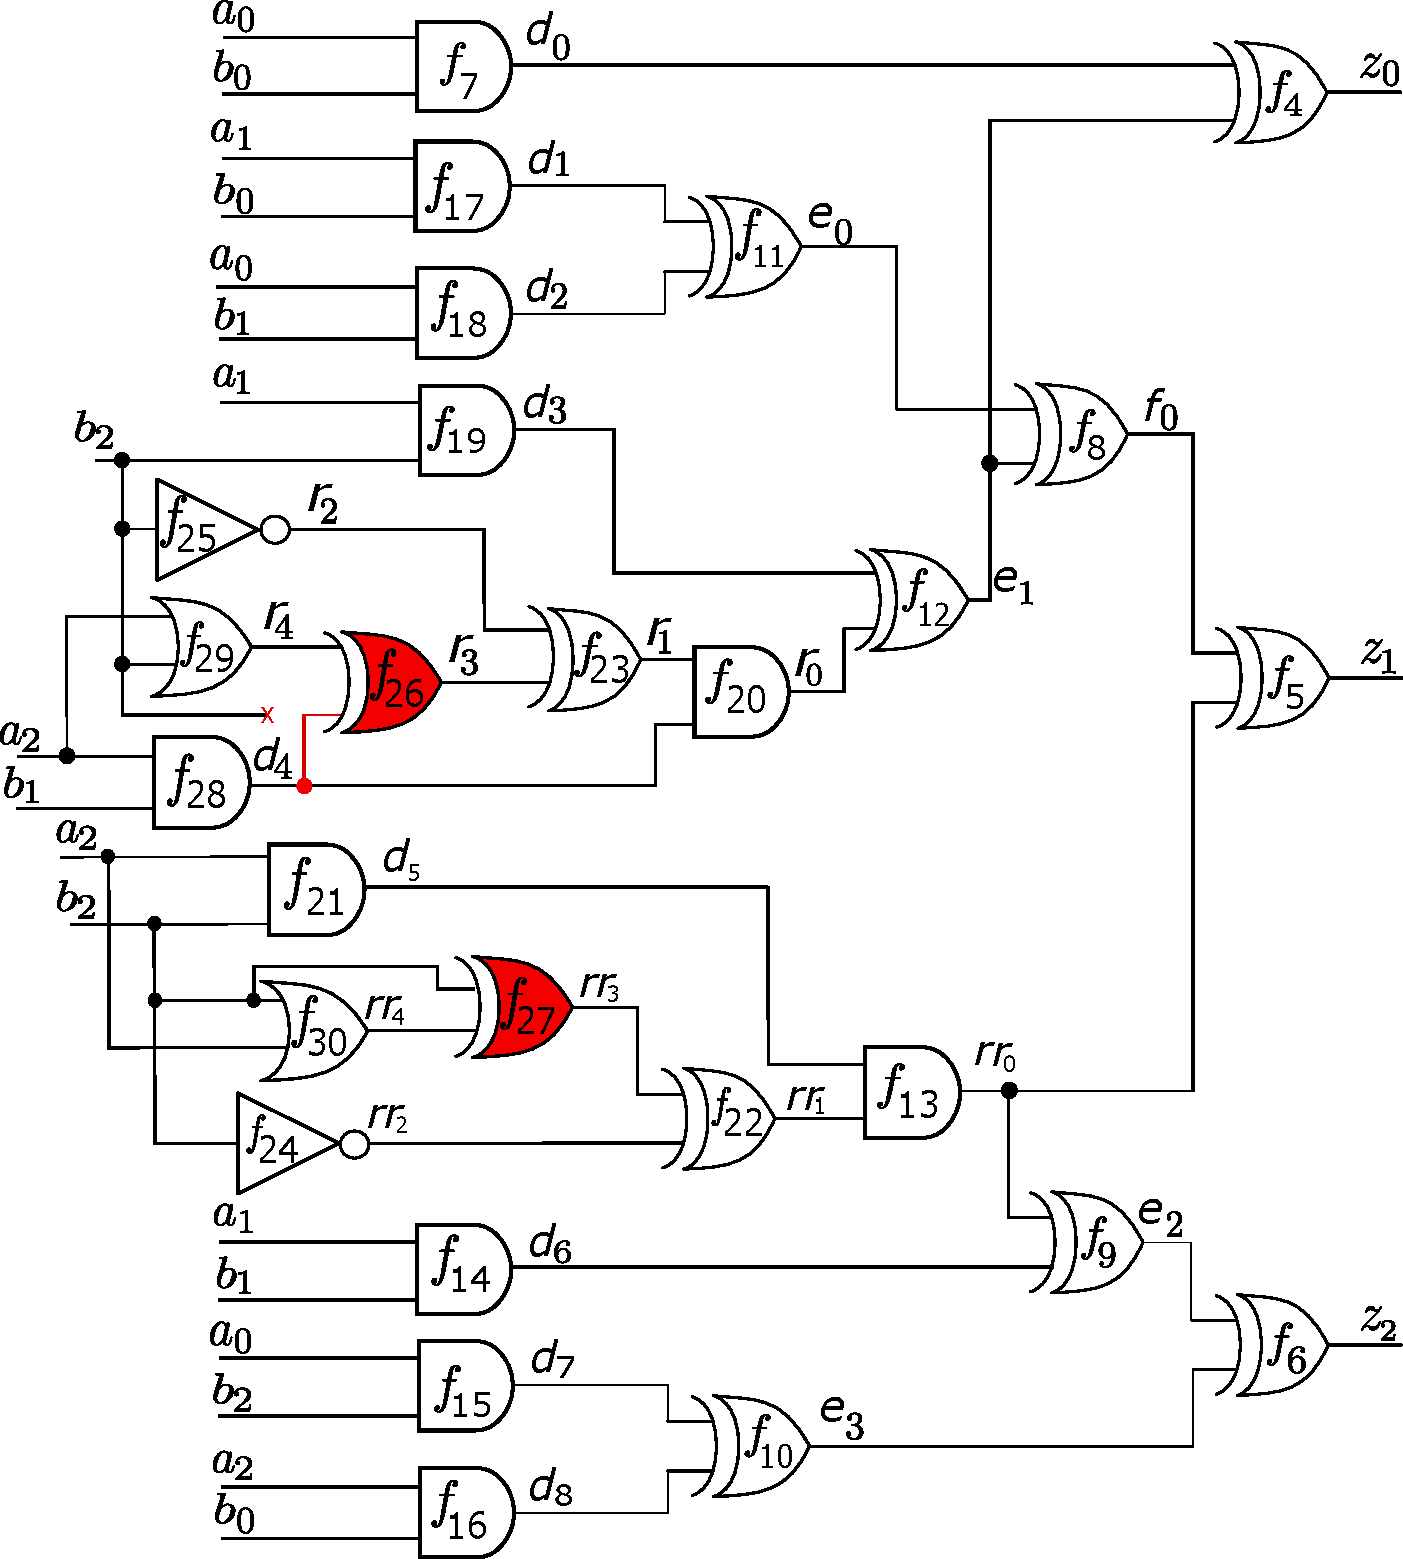
\includegraphics[scale = 0.29]{mas_3_ddc_mfr_a.pdf}
    \end{center}
    \Description{\caption{{\footnotesize  
        A faulty $\impl$ of the circuit $C$: a 3-bit finite
        field multiplier ($n$=3) with bugs introduced at net $r_3$
        (AND gate replaced with an XOR gate and one of the inputs
        mis-connected to $d_4$ instead of $b_2$) and net $rr_3$ (AND gate
        replaced with an XOR gate).}}}
    \caption{{\footnotesize  
        A faulty $\impl$ of the circuit $C$: a 3-bit finite
        field multiplier ($n$=3) with bugs introduced at net $r_3$
        (AND gate replaced with an XOR gate and one of the inputs
        mis-connected to $d_4$ instead of $b_2$) and net $rr_3$ (AND gate
        replaced with an XOR gate).}}  
    \label{fig:mas_bug_W}
    % \vspace{-0.25in}
\end{figure}

\section{Rectification Check}\label{sec:rcheck}

% The rectifiability check presented in~\cite{Vkrao:ISQED21} relies on the 
% results of the Strong Nullstellensatz over finite fields and \Grobner
% basis reduction $f\xrightarrow{GB(J+J_0)}_+ r$. 
% To help formulate the rectification function computation, we restate 
% the decision procedure presented in~\cite{Vkrao:ISQED21} as per our needs.
In~\cite{Vkrao:ISQED21}, the authors presented techniques 
which utilize the aforementioned polynomial ideal setup
to derive the necessary and sufficient conditions for the existence
of a multi-fix rectification at the given set of targets.
We rephrase and restate Thm. V.1 from~\cite{Vkrao:ISQED21}, and 
briefly discuss its key aspects. 
Subsequently, we formulate the computation of rectification functions by utilizing
the outcome of their decision procedure.
% Subsequently, we formulate the computation of rectification functions as a 
% quantification procedure by building upon
% the outcome of their decision procedure.

\begin{Theorem}{\bf [Multi-fix Rectification Theorem]}\label{Thm:rect}
A \spec~polynomial $f$, a faulty 
\impl~$C$ represented using the ideal 
$J +J_0 = \langle F \cup F_0\rangle \subset R$,
 and a set of targets $W=(w_1,\dots,w_m) \subset \{X-X_{PI}\}$
 are given. 
%  Here, each $w_i$, for $i=1,\dots,m$ represents the output
% of an $i^{th}$ gate in $C$.
% The targets in set $W$ are considered fan-in free or treated as pseudo primary inputs.
RTTO $>$ is imposed on $R$. Let $W_c = \{(0,0,..,0),\dots,(1,1,..,1)\},$ $~|W_c| = 2^m$, 
 denote the set of all possible $\{0,1\}$ assignments to targets $W$.
 This is akin to computing cofactors of the circuit functions with 
 respect to the targets $W$.
 % Roland et al.~\cite{MF_Huang:DATE12} refer to them as cofactors
 % and we use the same terminology. 
Each cofactor tuple $W_c[l]$ serves as one set
 of assignments to $m$ targets at their respective indexes in $W$. 
% We construct the ideals by considering all the
% t 
% Here $F=\{f_1,\dots,f_{w_1}:w_1+tail(f_{w_1}),\dots,f_{w_m}:w_m+tail(f_{w_m}),\dots,f_s\}$
%(Setup as described in Sec.\ref{sec:rsetup}),
The following ideals are constructed:  
\bi
\item {\small $J_l = \langle F_l\rangle =\langle f_1,\dots,f_{w_1}:w_1+W_c[l][1],
	\dots,f_{w_m}:w_m+W_c[l][m]$ $,\dots,f_s\rangle$}, $\forall l \in 1,\dots 2^m$. 
\ei

Reduce $f$ by $F_l\cup F_0$ to obtain remainders $rem_l$: 
$f\xrightarrow{F_l\cup F_{0}}_+ rem_l,$  for $1 \leq l \leq 2^m$.
Then, the circuit $C$ is rectifiable at the target set $W$ {\bf\textit{if
   and only if}} union of varieties $\bigcup\limits_{l=1}^{2^m}V(rem_l) = \Ftwo^{|X_{PI}|}$. 
\end{Theorem}

{\red
To synthesize a patch, a desired $u_i$ corresponds
to a polynomial function $u_i:\F_2^{|X_{PI}|} \mapsto \F_2$. 
\begin{Proof}
As the correction at target $W$ makes $C$ match $f$, $f$ should vanish on
$V_{\Fkk}(J')$.
Moreover, each $rem_l$ comprises only $X_{PI}$ variables. This is
because WRTO $>_R$ ensures that each non primary input variable (each gate
output and  word-level variable) appears as the leading term of some
polynomial in $F'$. Thus each non primary input variable is canceled
in the reduction $f\xrightarrow{F'_l, F'_{0}}_+ rem_l$. Furthermore,
as $X_{PI}$ take values in $\F_2$, $x^2=x, \forall x \in
X_{PI}$. Hence, 
% even though $V_{\Fkk}(J')$ is evaluated in $\Fkk$,
$V(rem_l) \subseteq \F_{2}^{|X_{PI}|}$. Thus, the rectification theorem
 can be equivalently stated as: ``$f$ vanishes on
\begin{small}
$V_{\Fkk}(J') \iff \bigcup\limits_{l=1}^{2^m}V(rem_l) = \Ftwo^{|X_{PI}|}$''.
\end{small} 

(i) {\bf To prove ``$\Rightarrow$''}: Let $x_{PI} \in \Ftwo^{|X_{PI}|}$ be an
assignment to the primary input variables of $C$. Every assignment
$x_{PI}$ results in a corresponding assignment $x_{int}$ 
to rest of the variables in $C$. For each such point $(x_{PI},x_{int})\in \Fkk$,
the target $W$ evaluates to one of the values in the list $\delta$,
i.e. $(0,1,\be,\dots,\beta^{2^m-2})$. When $W = 0$, $J'_1$ vanishes on
the point $(x_{PI},x_{int})$. Likewise, $J'_2$ vanishes on
$(x_{PI},x_{int})$ when $W = 1$, and so on. Since
$f\xrightarrow{F'_l\cup F'_0}_+rem_l,1 \leq l \leq 2^m$, and $f$ vanishes
on the point $(x_{PI},x_{int})$ to begin with, we obtain that for
every  primary input assignment $x_{PI}$, one of the $rem_l$ vanishes. This
implies that $ \bigcup\limits_{l=1}^{2^m}V(rem_l) = \Ftwo^{|X_{PI}|}$.

(ii) {\bf To prove ``$\Leftarrow$''}: Say there exists an assignment to the
primary inputs $x_{PI} \in \Ftwo^{|X_{PI}|}$ such that $rem_1$ vanishes on
$x_{PI}$, i.e. $rem_1(x_{PI})=0$. For the given point $x_{PI}$, the rest of the variables 
of $C$ get a corresponding assignment $x_{int}$. 
As $f\xrightarrow{F'_1\cup F'_0}_+ rem_1$, we have that $f$ is a member of the
ideal $J'_1 + J'_0 + \langle rem_1 \rangle$. Therefore, when
$rem_1(x_{PI})=0$, the ideal $J'_1$ also vanishes on $(x_{PI},x_{int}) \in \Fkk$
because the tuple $(x_{PI},x_{int})$ is a valid evaluation of the circuit.
Further, $J'_0$ by definition vanishes everywhere in $R'$. This implies that
$f(x_{PI},x_{int})=0$. The argument similarly holds for each
$rem_{l}$ vanishing on some $x_{PI}$. This proves that for all primary
inputs, if any $rem_l:1 \leq l \leq 2^m$ vanishes, then $f$ vanishes too; and 
that completes the proof.
\end{Proof}
 }

The above check for union of varieties can be performed 
% as $\prod_{l=1}^{2^m} rem_l\xrightarrow{J_{0}^{X_{PI}}}_+0?$ (cf. Section \ref{sec:prelim}).
as product of ideals, i.e. by checking if $\prod_{l=1}^{2^m} 
rem_l\xrightarrow{J_{0}}_+0$.
RTTO $>$ is known to have the property that makes the division 
$f\xrightarrow{F_l\cup F_{0}}_+ rem_l$ mimic gate level substitution
in polynomial algebra.
% RTTO $>$, $f\xrightarrow{F_l\cup F_{0}}_+ rem_l$ 
% mimics polynomial substitution. 
Thus, after reduction, 
all non-primary input variables in the circuit are canceled and the 
final remainder has only $X_{PI}$ variables in its support.

\begin{Example}
\label{ex:3}
{\it 
Continuing on with the Ex. \ref{verify_ex}, we
demonstrate the rectification check presented in~\cite{Vkrao:ISQED21}
for $W=(r_3,rr_3)$. 

Constructing the $J_l$ ideals:
\bi
\item {\small$J_1 = \langle F_1\rangle$, where $F_1[f_{26}: r_3+0],F_1[f_{27}: rr_3 + 0]$},$(r_3 =0, rr_3 = 0)$ 
\item {\small$J_2 = \langle F_2\rangle$, where $F_2[f_{26}: r_3+0],F_2[f_{27}: rr_3 + 1]$},$(r_3 =0, rr_3 = 1)$
\item {\small$J_3 = \langle F_3\rangle$, where $F_3[f_{26}: r_3+1],F_3[f_{27}: rr_3 + 0]$},$(r_3 =1, rr_3 = 0)$
\item {\small$J_4 = \langle F_4\rangle$, where $F_4[f_{26}: r_3+1],F_4[f_{27}: rr_3 + 1]$},$(r_3 =1, rr_3 = 1)$
\ei
Reducing the $\spec$ $f: Z+A\cdot B$ modulo these ideals, we get:
\bi
\item $rem_1 = f \xrightarrow[]{F_1\cup F_{0}}_+(\ga+1)a_2b_1b_2+(\ga^2+\ga)a_2b_2$
\item $rem_2 = f \xrightarrow[]{F_2\cup F_{0}}_+(\ga+1)a_2b_1b_2$
\item $rem_3 = f \xrightarrow[]{F_3\cup F_{0}}_+(\ga+1)a_2b_1b_2+a_2b_1 + (\ga^2+\ga)a_2b_2$
\item $rem_4 = f \xrightarrow[]{F_4\cup F_{0}}_+(\ga+1)a_2b_1b_2+a_2b_1$
\ei

When we compute $\prod_{l=1}^{2^m} 
rem_l\xrightarrow{J_{0}}_+$, 
 we obtain remainder 0, thus confirming
that the target set $W=(r_3,rr_3)$ indeed admits correction.
% Even though it is beyond the scope of this paper, $W=a_2b_1b_2+\be \cdot a_2b_2$ 
% is a polynomial which can be computed to rectify the circuit. 
% In fact, the rectification test also passes with nets $d_2$ and $d_5$;
% implying that we could have selected $w_0$ to be $d_2$ instead of $e_0$. 
% However, the rectification test fails when $w_0=d_0$ and
%  $w_1=d_5$. When the problem is formulated with these nets, $\prod_{l=1}^{4} 
%  rem_l\xrightarrow{J_{0}^{X_{PI}}}_+\al^9a_2b_1b_2+\al^{36}a_2b_2$  implying that
%  these nets do not admit correction.   
}
\end{Example}

% every $F_l\cup F_0$ forms a \Grobner basis in itself, and hence
% each corresponding $rem_l \in \Fkn[X_{PI}]$, and subsequently 
% $V(rem_l) \subseteq \F_{2}^{|X_{PI}|}$. 
% The authors in~\cite{Vkrao:ISQED21} limit their findings to 
% proving the {\it existence} of rectification functions by means of a check.
% However, on further investigation, one could
% use the information embedded within this check to 
% characterize the rectification functions.
The concepts presented in~\cite{Vkrao:ISQED21} are limited to
proving the {\it existence} of rectification functions.
However, our investigation further reveals that their result
can be extended to characterize the desired rectification functions.
Intuitively, the concept can be elaborated as follows.
The variety of $rem_l$ for any $l$ corresponds to the set of
all assignments to primary inputs $X_{PI}$ (minterms) where the
$\spec$ $f$ agrees with the $\impl$ $C$. Thus, the
condition of Thm.~\ref{Thm:rect} implies that the union of individual
varieties of $rem_l$'s comprises the set of all minterms where $f$ and $C$ evaluate the same. 
Thus, for every primary input assignment, {\it there exists} a cofactor tuple
assignment $W_c[l]$ to $W$ such that $f$ and $C$ match. Consequently, there
exists a set of functions $U = (u_1,\dots,u_m)$ that can be computed to 
rectify every error minterm. We exploit and explore this concept 
to compute rectification functions in the following section.


% To synthesize a patch, a desired $u_i$ corresponds
% to a polynomial function $u_i:\F_2^{|X_{PI}|} \mapsto \F_2$. 
% \begin{Proof}
% As the correction at target $W$ makes $C$ match $f$, $f$ should vanish on
% $V_{\Fkk}(J')$.
% Moreover, each $rem_l$ comprises only $X_{PI}$ variables. This is
% because WRTO $>_R$ ensures that each non primary input variable (each gate
% output and  word-level variable) appears as the leading term of some
% polynomial in $F'$. Thus each non primary input variable is canceled
% in the reduction $f\xrightarrow{F'_l, F'_{0}}_+ rem_l$. Furthermore,
% as $X_{PI}$ take values in $\F_2$, $x^2=x, \forall x \in
% X_{PI}$. Hence, 
% % even though $V_{\Fkk}(J')$ is evaluated in $\Fkk$,
% $V(rem_l) \subseteq \F_{2}^{|X_{PI}|}$. Thus, the rectification theorem
%  can be equivalently stated as: ``$f$ vanishes on
% \begin{small}
% $V_{\Fkk}(J') \iff \bigcup\limits_{l=1}^{2^m}V(rem_l) = \Ftwo^{|X_{PI}|}$''.
% \end{small} 

% (i) {\bf To prove ``$\Rightarrow$''}: Let $x_{PI} \in \Ftwo^{|X_{PI}|}$ be an
% assignment to the primary input variables of $C$. Every assignment
% $x_{PI}$ results in a corresponding assignment $x_{int}$ 
% to rest of the variables in $C$. For each such point $(x_{PI},x_{int})\in \Fkk$,
% the target $W$ evaluates to one of the values in the list $\delta$,
% i.e. $(0,1,\be,\dots,\beta^{2^m-2})$. When $W = 0$, $J'_1$ vanishes on
% the point $(x_{PI},x_{int})$. Likewise, $J'_2$ vanishes on
% $(x_{PI},x_{int})$ when $W = 1$, and so on. Since
% $f\xrightarrow{F'_l\cup F'_0}_+rem_l,1 \leq l \leq 2^m$, and $f$ vanishes
% on the point $(x_{PI},x_{int})$ to begin with, we obtain that for
% every  primary input assignment $x_{PI}$, one of the $rem_l$ vanishes. This
% implies that $ \bigcup\limits_{l=1}^{2^m}V(rem_l) = \Ftwo^{|X_{PI}|}$.

% (ii) {\bf To prove ``$\Leftarrow$''}: Say there exists an assignment to the
% primary inputs $x_{PI} \in \Ftwo^{|X_{PI}|}$ such that $rem_1$ vanishes on
% $x_{PI}$, i.e. $rem_1(x_{PI})=0$. For the given point $x_{PI}$, the rest of the variables 
% of $C$ get a corresponding assignment $x_{int}$. 
% As $f\xrightarrow{F'_1\cup F'_0}_+ rem_1$, we have that $f$ is a member of the
% ideal $J'_1 + J'_0 + \langle rem_1 \rangle$. Therefore, when
% $rem_1(x_{PI})=0$, the ideal $J'_1$ also vanishes on $(x_{PI},x_{int}) \in \Fkk$
% because the tuple $(x_{PI},x_{int})$ is a valid evaluation of the circuit.
% Further, $J'_0$ by definition vanishes everywhere in $R'$. This implies that
% $f(x_{PI},x_{int})=0$. The argument similarly holds for each
% $rem_{l}$ vanishing on some $x_{PI}$. This proves that for all primary
% inputs, if any $rem_l:1 \leq l \leq 2^m$ vanishes, then $f$ vanishes too; and 
% that completes the proof.
% \end{Proof}
 

%where the union of
%varieties corresponds to the product of ideals and is characterized by
%Strong Nullstellensatz over finite fields ({\red refer Strong
%  Nullstellensatz}). 
%% \begin{small}
%% \begin{align*}
%% &\bigcup\limits_{l=1}^{2^m}V(rem_l) =V_{\Ftwo}( \prod_{l=1}^{2^m}
%%   rem_l)= V_{\Ftwo}( \langle \prod_{l=1}^{2^m} rem_l \rangle +
%%   J_0^{X_{PI}} ) \\
%% & \quad\quad\quad\quad\quad\quad\quad\quad = V_{\Ftwo}(\langle \prod_{l=1}^{2^m} rem_l \rangle+ J_0^{PI})
%%   % V_{\Fqbar}(\langle r_1\cdot \dots r_{2^m} \rangle+ J_0^{PI}) \\
%% \end{align*}
%% \end{small}
%% Thus, to check for MFR at target $W$, we need
%% to check if $\prod_{l=1}^{2^m} rem_l\xrightarrow{J_{0}^{PI}}_+0$?  


% \begin{algorithm}\label{rect_flow_alg}
% \caption{Rectification of finite field arithmetic circuits}\label{pseudocode}
% \begin{algorithmic}[1]
% \Require $\spec:f, buggy~\impl: C$ modeled as a polynomial ideal $F=\{f_1\dots,f_s\}$ under $RTTO >$ 
% \Assume {$C$ doesn't admit single-fix rectification} //~\cite{Vkrao:FMCAD18}
% \Ensure {Rectification of $C$ to match $f$}
% \Procedure{$rectification$}{} 
% \State {remainder = $verify(f,F+F_0)$} // Sec.\ref{sec:verify}
% \State {$\Oa = analyze$(remainder)} //Sec. V.1~\cite{Vkrao:FMCAD18}
% \State {$\In = PotentialNets()$} //Sec.\ref{subsec:target_nets}
% \State {$m = 2$; rectified = $False; \mathcal{O}_A = \emptyset ; F_w = \emptyset$}
% \Do %1
% \State {$\Oa^i = uniquePartition(\Oa,m)$}\label{prtn}
% \If {$\Oa^i \notin \mathcal{O}_A$}
% \State {$\mathcal{O}_A=\mathcal{O}_A \cup \Oa^i$}
% \State {$\M^i = intersectionCover(\Oa^i)$}  
% \State {$f_w=pickTargets(\M^i,m)$}\label{ptrgt}
% \If {$f_w \notin F_w$}
% \State {$F_w=F_w \cup f_w$}
% \State {$MFRSetup()$} //Sec.\ref{subsec:comp_fwrk}
% \If {$MFRCheck(F')==0$} //Sec.\ref{sec:rcheck}
% \State {rectified = $True$}
% \State {patch = $rectFunction$()} //Sec.\ref{sec:rfunc}
% \Else
% \State {$goto~\ref{ptrgt}$}
% \EndIf
% \Else
% \State {$goto~\ref{prtn}$}
% \EndIf
% \Else
% \State $m++$
% \EndIf
% \doWhile {((!rectified) $\&\&$ $m \le |\Oa|$)} %1
% \State \Return patch
% \EndProcedure
% \end{algorithmic}
% \end{algorithm}

%  However, as discussed before, their variety 
% $V(rem_l)\subseteq \F_{2}^{|X_{PI}|}$. We can compute a polynomial $pr_l \in \F_{2}^{|X_{PI}|}$
%  such that $V(pr_l) = V(rem_l)$~\cite{Utkarsh:VLSI18}. 

% The authors discuss how rectifiability of $C$ against its 
% $\spec$ at a given set of $m$-distinct targets 
% $W=(w_1,\dots,w_m)\subset \{\{X\}-\{X_{PI}\}\}$ can be ascertained
% algebraically. 
%  
\section{Computing Rectification Functions}\label{sec:rfunc}

% The {\it multi-fix rectification theorem} determines whether there 
% exists a set of polynomial functions $U = (u_1,\dots,u_m)$  
% such that substituting every patch function $u_i$ as the $tail$ 
% at its respective target $w_i$, for $i = 1,\dots,m$, makes $C$ 
% functionally equivalent to $\spec$. 
% We formulate the computation of rectification function by extending 
% the decision procedure to a quantification 

For a given set of targets $W$, due 
to the presence of don't cares (DC), there may exist more 
than one set $U$ of rectification functions which will rectify the circuit.
In this section, we describe the notion of DC 
in the MFR setup which can be exploited for the simplification
of rectification patches.
Exploring all the DC conditions for $m$ targets might be computationally infeasible; we
present two different approaches to overcome this. First,
we present an approach to compute an on- and off-set for each rectification function by 
heuristically resolving all the DC conditions.
Following this, we present an approach to 
explore and compute a subset of the DC conditions, along with 
on- and off-sets, for each rectification function.

% In this section, we describe the notion of DC 
% in the MFR setup which can be exploited for further simplification
% of rectification patches.
% % for synthesis of efficient rectification patches.
% However, it is infeasible to explore and analyze all the possible DC-sets. 
% To overcome this complexity, we first present a 
% greedy heuristic which computes a rectification function 
% set $U$ by eliminating all the DC conditions.
% % We first present a greedy approach which quickly computes an on- and off-set for each rectification patch. 
% Following this, we present an approach to explore and compute a subset of 
% the DC conditions, along with on- and off-sets, for the given targets.

% \vspace{-0.2in}
% , such that substituting the patches
% into the polynomial set $F$ $(f_{w_1}:w_1+u_1,\dots,f_{w_m}:w_m+u_m)$ 
% rectifies the circuit.

% This involves computing a {\bf reduced \Grobner basis} for the polynomial $rem_l$ and then 
%  From the ideal $J$, a polynomial $U$ can be computed
% using Lagrange interpolation,
% which evaluates to 0 on $V(J)$ and 1 everywhere else $i.e.$ $V(U)=V(J)$. 
% % Due to the formulation of Lagrange interpolation, 
% The polynomial
% $U$ has variables in the set $\xpi$, and coefficients in $\{0,1\}$; $U \in \F_2[\xpi]$.
% Therefore, $U$ always evaluates to either 0 or 1 for any value of
% $\xpi$ variables. 

% After computing $\uc$, we can patch the circuit
% with the polynomial $f_i: x_i + \uc$.

% \subsection{Background}
% A \Grobner basis computed using Buchberger's algorithm is not a canonical
% representation of an ideal in itself. To obtain the canonical representation of
% an ideal, we need to compute a {\bf reduced \Grobner basis}. A reduced \Grobner basis
% is computed by first computing a minimal \Grobner basis, and then reducing it.

% \begin{Definition}\label{def:minigb}
% A {\bf minimal Gr\"obner basis} $G=\{g_1,\dots,g_t\}$ for a polynomial ideal $I$ is a \Grobner basis for $I$ such that
%     \begin{itemize}
%         \item $lc(g_{i})=1,\forall g_{i}\in G$
%         \item $\forall g_{i} \in G$,  $lt(g_{i}) \notin \langle lt(G-\{g_{i}\})\rangle$
%     \end{itemize}
% \end{Definition}
% A {\bf minimal} \Grobner basis is a \Grobner basis such that all polynomials
% have a coefficient of $1$ and no leading term of any element in $G$ divides 
% another in $G$.
% Given a \Grobner basis $G$, a minimal \Grobner basis can be
% computed as follows:
% \begin{enumerate}
% \item Make every $g_i \in G$ monic, i.e $g_i=g_i/lc(g_i)$
% \item For $g_i, g_j \in G$ where $i\neq j$, remove $g_i$ from $G$ if $lt(g_i)\mid lt(g_j)$, i.e. remove every polynomial in $G$ whose leading term is divisible by the leading term of some other polynomial in $G$.
% \end{enumerate}

% Then $G$ is minimal $w.r.t.$ number of elements. 
% A minimal Gr\"obner basis can then be further reduced.
% \begin{Definition}
%     A {\bf reduced Gr\"obner basis} for a polynomial ideal $I$ is a Gr\"obner basis $G=\{g_{1},\dots,g_{t}\}$ such that:
%     \begin{itemize}
%         \item $lc(g_{i})=1,\forall g_{i}\in G$
%         \item $\forall g_{i} \in G$, no monomial of $g_{i}$ lies in $\langle lt(G-\{g_{i}\})\rangle$
%     \end{itemize}
% \end{Definition}
% $G$ is a reduced Gr\"obner basis when no monomial of any element in $G$ is
% divisible by the leading term of another element. 

% \subsection{Computing Rectification Patches}
\subsection{Greedy Approach for MFR}\label{comp:GFC}

To illustrate the greedy approach, consider the case with $m = 2$, where $W_c = \{(0,0), (0,1), (1,0), (1,1)\}$, and we must compute rectification functions $u_1$ and $u_2$. For brevity, let $V_{W_c[i]} = V(rem_i)$, for $1 \leq i \leq 2^m$; in this case, $V_{(0,0)} = V(rem_1)$, $V_{(0,1)} = V(rem_2)$, and so on.

Recall that $V_{(0,0)}$ comprises the set of points where the $\impl$ and $\spec$ evaluate the same for the corresponding assignments $(0,0)$ to the targets. This implies that at these points, the rectification functions $u_1$ and $u_2$ should evaluate to $0$. Table~\ref{tab:tar_assign} shows the required evaluations of $u_1$ and $u_2$ for the points in each variety, following the same reasoning. The on-set of the rectification function for a target corresponds to the union of the varieties (sets) where the function evaluates to $1$, and the off-set corresponds to the union of the varieties (sets) where the function evaluates to $0$. In this case,
the on-set of $u_1$ consists of the set of points in $V_{(1,0)} \cup V_{(1,1)}$, and the off-set of $u_1$ consists of the set of points in $V_{(0,0)} \cup V_{(0,1)}$. Similarly, the on-set and off-set of $u_2$ consists of the points in $V_{(0,1)} \cup V_{(1,1)}$ and $V_{(0,0)} \cup V_{(1,0)}$, respectively. The functions $u_1$ and $u_2$ could be
synthesized using these on- and off-sets.

\begin{table}[hbt!]
  \centering
  \caption{Function evaluations }\label{tab:tar_assign}
  \begin{tabular}
    {!{\vrule width 1pt} c !{\vrule width 1pt} c | c !{\vrule width 1pt}}\noalign{\hrule height 1pt}
    {\textit Variety} & {$u_1$} & {$u_2$} \\ \noalign{\hrule height 1pt}
    $V_{(0,0)}$             & 0       & 0       \\ \hline
    $V_{(0,1)}$             & 0       & 1       \\ \hline
    $V_{(1,0)}$             & 1       & 0       \\ \hline
    $V_{(1,1)}$             & 1       & 1       \\ \noalign{\hrule height 1pt}
  \end{tabular}
\end{table}
    
However, the above argument is only correct when $V_{(0,0)}, V_{(0,1)}, $ $ V_{(1,0)}, V_{(1,1)}$ are pairwise disjoint, which may not be true in practice. For example, for a point contained in $V_{(0,0)} \cap V_{(0,1)}$, $(u_1,u_2)$ must evaluate either to $(0,0)$, or to $(0,1)$ in order for the $\impl$ to evaluate to the same value as the $\spec$; this point would be in both the on- and off-set of $u_2$ in the method previously described. A decision procedure is necessary to determine the evaluation of $(u_1,u_2)$ at these intersections. 
We present a greedy approach which resolves such ambiguities by imposing an order on the sets.
An example of our greedy approach to evaluate $(u_1,u_2)$ for an order $V_{(0,0)} > V_{(0,1)} > V_{(1,0)} > V_{(1,1)}$ is as follows:

% One complication arises from the fact that the intersections of these varieties might not be empty.  
% % These points are in the off-set of $u_1$, however, they are in the on-set and off-set of $u_2$
% Therefore, $u_1$ must evaluate to $0$, but $u_2$ may evaluate either to $0$ or to $1$; the choice will change the resulting patch function. For points in any intersection between any of the sets $V_{(0,0)}, V_{(0,1)}, V_{(1,0)}, V_{(1,1)}$, a similar choice must be made, resulting in an exponential number of potential distinct rectification functions.  A simple approach to overcome this complexity and construct a rectification function for each target is as follows: 

First, we place all the points from $V_{(0,0)}$ into the off-sets of $(u_1, u_2)$. Next, we place all the points from $V_{(0,1)} \setminus V_{(0,0)}$ into the off-set of $u_1$ and the on-set of $u_2$. We perform the set difference to avoid placing the points in $V_{(0,0)} \cap V_{(0,1)}$ into both the on-set and off-set of $u_2$. Next, we place all the points from $V_{(1,0)} \setminus (V_{(0,0)} \cup V_{(0,1)})$ into the on-set of $u_1$, and the off-set of $u_2$. Finally, we place the remaining points from $V_{(1,1)} \setminus (V_{(0,0)} \cup V_{(0,1)} \cup V_{(1,0)})$ into the on-set of $(u_1, u_2)$.
% \begin{figure}[hbt]
%     \begin{center}
%     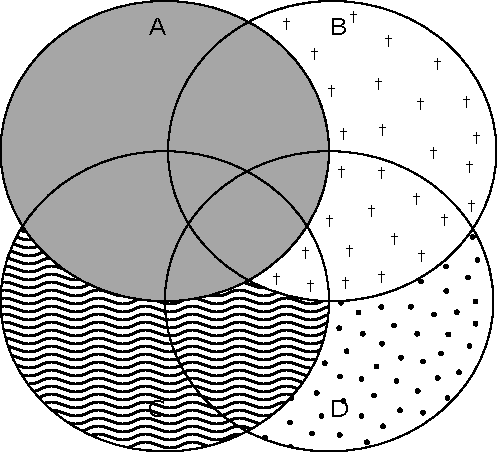
\includegraphics[scale = 0.31]{simple_rect_func1.pdf}
%     \end{center}
%     \caption{{\footnotesize  
%       Rectification function computation
%       illustrated for two targets}}  
%     \label{fig:simp_rec_func}
%     % \vspace{-0.25in}
% \end{figure}
% Thus, for a target $u_i$, the on-set corresponds to the union of the sets where $u_i$ evaluates to $0$, 
% and the off-set corresponds to the union of the sets where $u_i$ evaluates to $1$. 
The resulting on- and off-sets for $u_1$ and $u_2$ are shown below.

\begin{small}
\begin{align*}
  \begin{split}
    V(u_{1_{on}})&= (V_{(1,1)} \setminus (V_{(0,0)} \cup V_{(0,1)} \cup V_{(1,0)})) \cup (V_{(1,0)} \setminus (V_{(0,0)} \cup V_{(0,1)}))\\
    V(u_{1_{off}}) &= (V_{(0,0)}) \cup (V_{(0,1)} \setminus V_{(0,0)}) \\
    V(u_{2_{on}})&= (V_{(0,1)} \setminus V_{(0,0)}) \cup (V_{(1,1)} \setminus (V_{(0,0)} \cup V_{(0,1)} \cup V_{(1,0)}))\\
    V(u_{2_{off}}) &= (V_{(0,0)}) \cup (V_{(1,0)} \setminus (V_{(0,0)} \cup V_{(0,1)}))
  \end{split}
\end{align*}
\end{small}

This approach with the given order greedily places points into the off-sets of the rectification functions $(u_1, u_2)$ where possible, and only places points into the on-sets of the rectification functions when necessary. 
Subject to the given order, the on-sets of the rectification functions are thus minimized. For the experiments in this paper, we always use the order
$V_{W_c[i]} > V_{W_c[j]}$ for $i < j$, as in the above example, though any order would yield valid rectification functions. 

Generalizing our greedy approach for $m$ targets, we first
construct the following composite sets (varieties):
\begin{equation}
  \label{eqn:composite_greedy}
  S_l=
  \begin{cases}
    V_{W_c[1]},                                                & \text{if}\ l=1   \\
    V_{W_c[l]} \setminus (\bigcup\limits_{j=1}^{l-1}V_{W_c[j]}), & 2\leq l \leq 2^m
  \end{cases}
\end{equation}

The resulting on-set and off-set functions for each target $i$, where $1 \leq i \leq m$ are: 
\begin{align}
  \label{eqn:ui_on_off}
  \begin{split}
  V(u_{i_{on}}) &= \bigcup S_l,~\forall l~|~W_c[l][i]=1 \\
  V(u_{i_{off}}) &= \bigcup S_l,~\forall l~|~W_c[l][i]=0
  \end{split}
\end{align}

% Vikas, can you help me write this paragraph? Something about how 
% 1. this gives us the varieties of u_i, but we can't find those directly, so instead we use
% the product of rem_l's and colon ideals to find the set unions and differences and end up with a polynomial
% whose variety is V(u_ion), V(u_ioff). Or something like that. 



% Since the approach resolves all the DC conditions instantly, the computed composite sets $S_l$ 
% are pairwise disjoint. As a result, the on- and off-sets for each target are 
% complements of each other. Hence, one can 
% use either $u_{i_{on}}$ or the complement of $u_{i_{off}}$ for patch function computation.

\subsection{Don't Care Conditions for MFR}\label{comp:DFC1}

% is agnostic to the synthesis cost of $\impl$
% However, we will introduce the notion of word-level don't cares 
% in the MFR setup, which can be further leveraged towards computing a desired solution.
% We want to select a rectification function which has the least synthesis cost 
% (in the number of literals or in the number of AND-XOR operations etc.). 

% Although the greedy approach yields a correct rectification function, it does not compute any Don't Care (DC) conditions, but instead heuristically assigns points to the off-set when possible at the intersections of varieties. 
% DC conditions can be exploited to synthesize efficient patch functions. In this section, we explore the sets of points where DC conditions appear and propose an approach to systematically compute a subset of these DC points for each target.

% For a given target $W$, due to the presence of Don't care (DC), there may exist more 
% than one rectification function ($U$) which will rectify the circuit.
% The choice of these rectification functions can have significant synthesis consequences.
% As shown above, the simple approach presented on computing a rectification 
% function completely eliminates these DC conditions.
% Exploring the complete DC sets for simplification of a rectification function is
% a logic optimization problem and is beyond the scope of this paper.
% However, we will describe and show the existence of DC sets 
% in the MFR setup which can be utilized to converge towards a desired solution.
% , we will introduce the notion of word-level don't cares in the MFR setup.

% \subsubsection{Strong and Conditional Don't Care Conditions}

% We define two distinct types of DC points for circuits with multiple rectification targets: strong don't care ($DC_{st}$) points and conditional don't care ($DC_{cond}$) points. Strong don't care points for a target are defined as the points where the $\impl$ and $\spec$ match when the target evaluates either to $0$ or to $1$ at those points, independent of the evaluations of other targets at those points. By contrast, conditional don't care points for a target are the points where the $\impl$ and $\spec$ match when the target evaluates either to $0$ or to $1$, but where the choice is conditioned on the evaluations of other targets at those points.

% An intersection of varieties contain DC points for a set of rectification functions $u_i, \dots, u_j$ if 1. Every binary combination of evaluations of $u_i, \dots, u_j$ results in $C$ matching the $\spec$, where 2. The remaining rectification functions evaluate either to $1$ or to $0$ for every combination of evaluations of $u_i, \dots, u_j$. 

% For example $V_{(0,0,0)} \cap V_{(0,0,1)} \cap V_{(0,1,0)} \cap V_{(0,1,1)}$ contains DC points for u_2, and u_3, but 
% $V_{(0,0,0)} \cap V_{(0,0,1)} \cap V_{(0,1,0)} \cap V_{(1,1,1)}$ doesn't - it violates #2.
%

Let $U_d \subseteq U$ denote a subset of the target rectification functions. 
We are interested in the DC conditions which arise for these functions at 
points where they may evaluate to any value, for some fixed 
evaluation of the remaining functions in the set $\{U \setminus U_d\}$. 
% Such points exist only at the intersections of varieties.
For example, consider a point in $V_{(0,0)} \cap V_{(0,1)}$ for 
a circuit with two targets. As discussed previously, $u_1$ must evaluate to $0$ at 
this point, but $U_d = \{u_2\}$ may evaluate either to $0$ or to $1$,
so this is a $DC$ point for $u_2$. 


% We will continue with the illustration of $m=2$ with $U=\{u_1,u_2\}$, 
% and let $U_d=\{u_2\}$. The don't care conditions for $u_2$ are the points 
%  Continuing with the $m=2$ 
% illustration, the entire DC condition evaluations for the functions $(u_1,u_2)$ are 
% given as $DC = \{(0,d),(d,0),(d,1),(1,d),(d,d)\}$. Here,
% $d \in \{0,1\}$ denotes a don't care evaluation.
% Not really sure how to talk about these intersections....
Not every intersection of varieties yields $DC$ points 
which follow the conditions described above. 
Consider a point in $V_{(0,0)} \cap V_{(1,1)}$. Here, $(u_1, u_2)$ 
must evaluate either to $(0,0)$ or to $(1,1)$. If this point were 
assigned to the $DC$ set of $u_2$, for example, the $\spec$ and $\impl$ 
would only evaluate the same if $u_1$ evaluated to the same value as $u_2$.  
Thus, $u_1$ would become a function of $u_2$ at this point. This point 
cannot be placed into the on-set, off-set, or DC-set of $u_1$ before $u_2$ 
is evaluated. To avoid inter-dependencies between the rectification functions, we do not classify 
points in such intersections as $DC$ points. We rely on our greedy heuristic to 
evaluate these points. 
% In contrast, in the previous 
% case, $u_1 = 0$ and $u_2 = DC$ for a point in $V_{(0,0)} \cap V_{(0,1)}$. 

% Instead, we can use a heuristic to make a decision to place 
% points in this intersection into the off-set or on-set of both $u_1$ and $u_2$. 
% These constitute $DC_{cond}$ points for both targets because the targets individually may evaluate either to $0$ or to $1$, with the condition that they evaluate to the same value as the other target. 

% Further, some intersections might involve more than two varieties. The intersection 
% $V_{(0,0)} \cap V_{(0,1)} \cap V_{(1,0)} \cap V_{(1,1)}$ constitutes a $DC$ 
% set for both $u_1$ and $u_2$ because at this intersection, every combination 
% of evaluations $(0,0), (0,1), (1,0), (1,1)$ results in the $\spec$ and $\impl$ agreeing. 

Finally, consider a point in $V_{(0,0)} \cap V_{(0,1)} \cap V_{(1,0)}$. 
This point cannot be a DC point for both targets simultaneously 
since the evaluation $(1,1)$ here will result in an incorrect rectification function. 
However, because $V_{(0,0)} \cap V_{(0,1)} \cap V_{(1,0)} \subset V_{(0,0)} \cap V_{(0,1)}$, 
we could treat this point as a $DC$ point for $u_2$ and evaluate $u_1$ to $0$. 
Alternatively, because $V_{(0,0)} \cap V_{(0,1)} \cap V_{(1,0)} \subset V_{(0,0)} \cap V_{(1,0)}$, 
we could treat this point as a $DC$ point for $u_1$ and evaluate $u_2$ to $0$.
Thus, we have a choice to place this point in the $DC$-set of either targets, but not both. 

% In the next section we describe a heuristic to make decisions for points in intersections such as these.

% is not an $DC_{st}$ set for $u_1$ or $u_2$  Instead, this intersection represents a set of $DC_{cond}$ points for both targets because each target individually may evaluate to $0$ or to $1$, with the condition that both targets may not evaluate to $1$. However, because $V_{(0,0)} \cap V_{(0,1)} \cap V_{(1,0)} \subset V_{(0,0)} \cap V_{(0,1)}$, we can treat these points as $DC_{st}$ points for $u_2$ and evaluate $u_1$ to $0$. Alternatively, because $V_{(0,0)} \cap V_{(0,1)} \cap V_{(1,0)} \subset V_{(0,0)} \cap V_{(1,0)}$, we could treat these points as $DC_{st}$ points for $u_1$ and evaluate $u_2$ to $0$. An intersection with $DC_{cond}$ points may or may not be contained in an intersection with $DC_{st}$ points. 

Finding every intersection containing $DC$ points for every target 
can be very expensive for circuits with more than a few targets. 
We therefore propose an approach to compute a subset of the $DC$ points by considering
only the set of pairwise intersections of varieties which contain $DC$ points for exactly one target, denoted as $DC_{pair}$.

% We therefore propose 
% an approach to compute a subset of the $DC$ points for each target. 
% We compute intersections of pairs of varieties which contain $DC$ points for exactly one target.

Let $d(W_c[j], W_c[k])$ denote the Hamming distance between the cofactor tuples $W_c[j]$ and $W_c[k]$. We compute the set of varieties which contain $DC$ points for one target, denoted $DC_{pair}$, from the equation below, where $1 \leq j,k \leq 2^m$.

\begin{equation}
  \label{eqn:dc_pair}
  DC_{pair} = \{V_{W_c[j]} \cap V_{W_c[k]}~|~d(W_c[j],W_c[k]) = 1\}
\end{equation}

Since the Hamming distance $d = 1$ between the cofactor tuples $W_c[j]$ and $W_c[k]$ for each intersection of varieties in $DC_{pair}$, exactly one rectification function may evaluate either to $0$ or to $1$. The remaining rectification functions require fixed evaluations of $1$ or $0$. Therefore, each intersection of varieties in $DC_{pair}$ yields $DC$ points for exactly one rectification function in $U$, and either on- or off-set points for the remaining rectification functions in $U$. We use $DC_{pair}$ to compute the $DC$ points for each rectification function, as described in the next section. 

% There exist $m*2^{(m-1)}$ such pairwise intersections which contain $DC$ points for one target. Depending on the circuit, the nature and position of the bugs, and the number of targets, however, finding each of these pairwise intersections may be infeasible. For this reason, we begin by finding only $m$ such intersections, one intersection for each target. We do this by computing the intersection of the variety corresponding to cofactor tuple $V_{W_c[1]}$, which corresponds to an assignment of $0$ to each target, with each variety whose cofactor tuple contains only one $1$ assignment, e.g. $V_{(0,0,0)} \cap V_{(0,0,1)}$. Points in these intersections correspond to off-set points for all but the target which may be assigned to $1$ or to $0$. If we successfully compute each of these $m$ intersections before a specified timeout, we may continue to compute the remaining pairwise intersections of varieties to find more $DC$ conditions. 

% % Should we describe here how we can look at groups of 4, 8, ... 2^m to find more DC conditions? I'm just not sure how to correctly describe a "group." I don't really want to bring up K-maps.

% Alternatively, if we are able to compute each pairwise intersection before the specified timeout, we may continue looking for more intersections which yield $DC$ points. We continue by computing intersections of four varieties. An intersection of four varieties constitutes a set of $DC$ points for two targets if for those targets every binary combination of target assignments results in the $\spec$ and $\impl$ agreeing, while the remaining assignments take the same constant value for each combination. For example, for $m = 3$, $V_{(0,0,0)} \cap V_{(0,0,1)} \cap V_{(0,1,0)} \cap V_{(0,1,1)}$ comprises a set of $DC$ points for $u_2$ and $u_3$; these points are off-set points for $u_1$. However, $V_{(0,0,0)} \cap V_{(0,0,1)} \cap V_{(1,1,0)} \cap V_{(1,1,1)}$ does not comprise a set of $DC$ points. If we were to put these points into the $DC$ set of $u_2$ and $u_3$, an incorrect rectification function might result if $u_1$ does not take the proper value for each evaluation of $u_2$ and $u_3$. If we successfully compute every intersection of four varieties, time permitting, we continue by looking at intersections of eight varieties, then sixteen, up to intersections of $2^m$ varieties. Points located in the intersection of all $2^m$ varieties are always $DC$ points for every target.

\subsubsection{Computing Rectification Functions with Don't Cares}\label{comp:DFC2}

Once the set $DC_{pair}$ has been found, a few steps remain to compute the on-, off-, and don't-care sets for each target. First, we follow an approach identical to the greedy approach to evaluate points not located inside $DC_{pair}$. We construct new composite sets $S_l^d$ for $1 \leq l \leq 2^m$, which are identical to the composite sets (varieties) created for the previous approach, except that all the points from $DC_{pair}$ set are removed.

\begin{equation}
  \label{eqn:composite_dc}
  S_l^d=
  \begin{cases}
    V_{W_c[1]} \setminus DC_{pair},                                                & \text{if}\ l=1   \\
    V_{W_c[l]} \setminus ((\bigcup\limits_{j=1}^{l-1}V_{W_c[j]}) \cup DC_{pair}), & 2\leq l \leq 2^m
  \end{cases}
\end{equation}

Points in these composite sets are assigned to the on- and off-set for each rectification function in the same way as 
Eqn.~(\ref{eqn:ui_on_off}), substituting $S_l$ with $S_l^d$.

Next, we must evaluate points within $DC_{pair}$ as on-, off-, or $DC$ points for each rectification function. We select the first pairwise intersection of varieties in $DC_{pair}$ and assign the points according to the cofactor tuples, as described previously. Since the intersections within $DC_{pair}$ may not be disjoint, we then take the next pairwise intersection, remove the points from the first intersection which have already been assigned, then assign these points according to the cofactor tuples. We continue this for each subsequent intersection of varieties from $DC_{pair}$, remembering to remove all previously assigned points at each step.

For example, for a circuit with two targets, $DC_{pair} = \{V_{(0,0)} \cap V_{(0,1)}, V_{(0,0)} \cap V_{(1,0)}, V_{(0,1)} \cap V_{(1,1)}, V_{(1,0)} \cap V_{(1,1)}\}$. We place the points in $V_{(0,0)} \cap V_{(0,1)}$ into the off-set of $u_1$ and the $DC$ set of $u_2$. We then place the points in $V_{(0,0)} \cap V_{(1,0)} \setminus V_{(0,0)} \cap V_{(0,1)}$ into the $DC$ set of $u_1$ and the off-set of $u_2$. We place points in $V_{(0,1)} \cap V_{(1,1)} \setminus ((V_{(0,0)} \cap V_{(0,1)}) \cup (V_{(0,0)} \cap V_{(1,0)}))$ into the $DC$ set of $u_1$ and the on-set of $u_2$. Finally, we place points in $V_{(1,0)} \cap V_{(1,1)} \setminus ((V_{(0,0)} \cap V_{(0,1)}) \cup (V_{(0,0)} \cap V_{(1,0)}) \cup (V_{(0,1)} \cap V_{(1,1)}))$ into the on-set of $u_1$ and the $DC$ set of $u_2$. 
Following this approach, we calculate on- off- and $DC$ sets for each rectification function. 


% We combine the on- and off-sets computed from $DC_{pair}$ to the on- and off-sets computed from the composite sets $S_l^d$ to find the complete on- and off-sets for each target. 
% a set of all the pairwise intersections of varieties which contain $DC$ points for one target, which we denote $DC_{pair}$. Let $d(V_i), V_j))$ denote the Hamming distance between the target assignments used during the computation of $V_i$ and $V_j$. We compute the set DC as follows:

% We follow the greedy approach to evaluate the rectification functions at the points not found in this DC set. We construct composite sets equivalent to those in equation \ref{eqn:composite_greedy}, but from which the points in the $DC$ set are removed, and assign these points to the on- and off-sets for the rectification functions in exactly the same manner as before. 

% \begin{equation}
%   \label{eqn:composite_DC}
%   S_{DC}=
%   \begin{cases}
%     V_{(0,0)} \setminus DC_U,                                                & \text{if}\ l=1   \\
%     V_l \setminus DC_U \setminus (\bigcup\limits_{j=1}^{l-1}V_j) & 2\leq l \leq 2^m
%   \end{cases}
% \end{equation}

% The $DC_{pair}$ set contains points which are $DC_{st}$ points for at least one target; these points may also be on- or off-set points for other targets. The intersections in $DC_{pair}$ also might not be pairwise distinct. We begin with the first set in $DC_{pair}$ 

% Computing every set containing SDC points for every target is very expensive for circuits with more than a few targets. Furthermore, experiments have shown that for many finite field arithmetic circuits, the intersections of four or more varieties is often very small or empty. For these reasons, we propose an approach to compute a subset of SDC points by considering only the intersections of pairs of varieties.
\subsection{Synthesizing Rectification Functions}\label{comp:synth}

The above techniques show how to construct a rectification function
by reasoning about the varieties of $rem_l$.  
% The techniques described above evaluate a unknown rectification
% function $u_i$ by reasoning about its variety, and the variety of the remainders $rem_l$.
However, algebraically, we compute these functions using their corresponding ideals.
Specifically, we show how the remainders computed in Thm.~\ref{Thm:rect} can be utilized for rectification function computation.
Even though the remainders $rem_l$ have coefficients in $\Fkn$ (higher field), their varieties 
are in $\F_{2}^{|X_{PI}|}$ as they correspond to bit-level assignments to $X_{PI}$. However, in~\cite{Utkarsh:VLSI18}, it was 
shown that it is a property of such ideals ($\langle rem_l, J_0 \rangle$) that their reduced
\Grobner bases (Def.~\ref{def:rgb}) have coefficients only in $\Ftwo$.
Further, it was shown that, given an ideal $I$ with coefficients in $\Ftwo$ with generators  $\{g_1,\dots,g_t\}$, 
a polynomial $p$ can always be constructed as $p = (1+g_1)(1+g_2)\dots(1+g_t)+1$, such that $V(p) = V(I)$. 
% This helps in computing a singleton polynomial for each 
%% {\it Ideal-Poly Conversion:} Over finite fields, given an ideal $J$, 
%% a polynomial $p$ can always be computed 
%% such that $V(p) = V(J)$. Let $\{g_1,\dots,g_t\}$ denote the generators
%% of $J$. Then, the polynomial $p$ can be constructed as, 
%% $p = (1+g_1)(1+g_2)\dots(1+g_t)+1$~\cite{Utkarsh:VLSI18}. 
% i.e. $V(rem_l)\subseteq \F_{2}^{|X_{PI}|}, 1 \leq l \leq 2^m$.
% It is a property of such ideals ($\langle rem_l,\jzxpi \rangle$), that their Reduced
% \Grobner basis (Def.~\ref{def:rgb}) will have coefficients only in $\Ftwo$.
% Once we compute a GB with coefficients in $\Ftwo$, we can translate it to a polynomial 
% which has the same variety as the ideal (Sec.~\ref{sec:prelim}).
Consequently, the rectification function operations are restricted to
algebraic computations in $\F_2[X_{PI}]\equiv \B$. 

To compute the patch $u_i$, we perform the following steps:
\bi
\item Compute reduced \Grobner bases of $\langle rem_l, J_0 \rangle$.
\item Construct a singleton polynomial $p$ such that \\ $V(p) = V(\langle rem_l, J_0 \rangle)$.
\item Impose an order on the sets for $DC_{pair}$ and composite set computations.
\item Compute $DC_{pair}$ using Eqn.~(\ref{eqn:dc_pair}), and then obtain the composite sets
      in Eqn.~(\ref{eqn:composite_dc}) which are then assigned to DC-, on- and off-sets of the 
      rectification functions (Sec.~\ref{comp:DFC1}).
\item In order to perform the variety union, intersection, and difference operations, we use ideal 
        product, sum, and colon operations, respectively, on the
        singleton polynomial $p$ representation of the ideal.
% Use ideal operations sum, product, and colon ideal to perform intersection, 
% sum, and difference of varieties, respectively.
\item The above procedure delivers $u_{i_{DC}}$ and $u_{i_{on}}$ as singleton polynomials in $\Ftwo[X_{PI}]$.
Translate $u_{i_{DC}}$ and $u_{i_{on}}$ into Boolean functions by interpreting the product, sum,
and '+1' as Boolean AND, XOR, and INV gates, respectively. Optimize the on-set $u_{i_{on}}$ w.r.t. to the DC-set $u_{i_{DC}}$.
\ei

%  A polynomial in $\F_2[X_{PI}]$ can be converted to a Boolean AND-XOR operation. This expression can be
% synthesized into a sub-circuit whose output can be connected to the respective targets in $W$ to rectify the circuit.
% As the product and sum operations are performed modulo 2, they can be implemented
% in a circuit using AND and XOR gates, respectively.

% The expression can be synthesized into a sub-circuit by replacing the modulo 2 product and sum 
% in the polynomial expression with the Boolean AND and XOR operators, respectively.
% We synthesize a sub circuit by interpreting sum as XOR $\pmod{2}$ and product 
% as AND gates.
% Subsequently,  we convert the polynomial to corresponding Boolean functions by treating $+,\cdot,+1$ 
% as XOR, AND, and INV operations, respectively.

% In order to compute a desired $u_i \in \F_2[X_{PI}]$ with a 
% $\F_2^{|X_{PI}|} \mapsto \F_2$ mapping,
% we perform the following steps.


% \bi
% \item Compute the generators $Gr_l$ for the ideal $Jr_l=\langle rem_l \rangle$ as 
% $redGB(Jr_l+\jzxpi)$, where $rem_l \in \Fkn[X_{PI}]$.
% Then the polynomials in $Gr_l$ have coefficients in $\F_2$,
% and variables in $\xpi$[Corollary~8.1]~\cite{UTK:thesis}.
% \item Use the Ideal-Poly conversion procedure from (Section \ref{sec:prelim})
% to compute a polynomial $rem_l'$. The computed $rem_l'$ is such that 
% $rem_l'\in \F_2[X_{PI}]$ and $V(rem_l') = V(rem_l)$.
% \item To compute $u_i$ algebraically, we utilize the relevant ideal operations described in
% the ideal-variety correspondences (Section \ref{sec:prelim}) to perform the union, intersection,
% and set difference of varieties over $V(rem_l')$.
% \ei


% $U_{dc} = \bigcap\limits_{l=1}^{2^m}V(pr_l)$

% \begin{Example}
% Continuing with our example~\ref{ex:4}, for the circuit shown in Fig.~\ref{fig:mas_bug_W},
% the intersection of Variety of remainders yields us the DC for all the targets.

% $U_{dc} = \bigcap\limits_{l=1}^{4}V(pr_l) = a_2b_1b_2+a_2b_1+a_2b_2+1$
% \end{Example}

% However, our experiments show that for large class of benchmarks depending on the
% target selection, the intersection of all sets is most likely to be empty. Thus,
% we need a stronger DC set computation for individual targets.

% Recall that the variety of each $pr_l$ corresponds to the set of correct points
% for a given tuple assignment to the targets from $W_c[l]$. Thus, all 
% the points which lie in the intersection of all the $pr_l$'s comprises the 
% DC for all the targets.
% We can compute a polynomial $pr_l \in \F_{2}^{|X_{PI}|}$
%  such that $V(pr_l) = V(rem_l)$~\cite{Utkarsh:VLSI18}. 
% \subsubsection{DC for individual targets}

\begin{Example}\label{ex:4}
  Continuing with Ex.~\ref{ex:3}:
  % , we illustrate the above procedure:

  \bi
  \item $rem_3 = (\ga+1)a_2b_1b_2+a_2b_1 + (\ga^2+\ga)a_2b_2$ %\\ coefficients in $\Fkn$
  \item $redGB(\langle rem_3,J_0\rangle) = \{a_2b_1,a_2b_2\}$ %\\ coefficients in $\Ftwo$
  \item $p_{rem_3} = (1+a_2b_1)*(1+a_2b_2)+1 = a_2b_1b_2+a_2b_1+a_2b_2$
  \bi
    \item Here, $V(p_{rem_3}) = V(\langle rem_3, J_0 \rangle)$
  \ei
  \item Similarly, polynomials $p_{rem_l}$ for each $rem_l$ can be computed.
  \ei
  The rectification polynomials for the targets $(r_3,rr_3)$ computed using the greedy approach~(Sec.~\ref{comp:GFC})
  \begin{align*}
    % \begin{split}
      &u_{1_{on}}  = a_2b_1b_2; &u_{1_{off}} &= a_2b_1b_2 +1; &r_3  &= u_{1_{patch}} =(a_2\wedge b_1 \wedge b_2);\\
      &u_{2_{on}}  = a_2b_2;    &u_{2_{off}} &= a_2b_2+1;     &rr_3 &= u_{2_{patch}}= (a_2\wedge b_2).
    % \end{split}
  \end{align*}
  The rectification polynomials for the targets $(r_3,rr_3)$ computed using the on-set and don't care simplification~(Sec.~\ref{comp:DFC2})
  \begin{flalign*}
    % \begin{split}
     &u_{1_{dc}} = a_2b_1b_2+a_2b_2;&u_{1_{on}} &= a_2b_1b_2; &r_3 &= u_{1_{patch}} = a_2\wedge b_2; \\
     &u_{2_{dc}} = a_2b_2+1;        &u_{2_{on}} &= a_2b_2;    &rr_3 &= u_{2_{patch}} = 1. 
    % \end{split}
  \end{flalign*}
  % As seen above, the synthesis tool ({\it sis}) was able to simplify 
  % the on-set for $u_1$ patch function.
\end{Example}



\section{Efficiency improvement using ZDDs}\label{impl}

The techniques described in rectification check and function computation 
predominantly involve \Grobner basis computations and polynomial reductions.
By virtue of RTTO $>$, the complexity of remainder ($rem_l$) generation 
in the rectification check was moved from one of computing GB to that of 
GB-reduction by way of multivariate polynomial division. 
However, the function computation operation also involves computing
a reduced GB, which can be especially prohibitive when applied to circuits with
large size operands. Hence, there is a need for efficient representation 
to overcome the infeasibility of these operations using conventional 
computer algebra tools. 
 
 As the GB algorithms are employed to compute rectification function
patches via remainders generated from the circuit, we analyze the circuit and its 
topology to derive specific
information, which we use to guide the computation of patches efficiently. Moreover, we
further show how our ZDD based algorithms can effectively utilize this information
to compute rectification patches. By combining our theories and algorithms, we can explore
the space of all possible rectification functions through their ON-set, OFF-set, and DC-set
of corresponding Boolean functions.

In this regards, we take inspiration from~\cite{Utkarsh:TCAD19} and utilize 
PolyBori’s~\cite{pbori:JSC09} reduction procedure with 
ZDDs~\cite{Minato:DAC93,Minato:DAC94} as the underlying data structure 
to improve our proposed approach.
PolyBori proposed the use of ZDDs to compute
\Grobner bases for Boolean polynomials. PolyBori is a generic Boolean GB computational
engine that caters to many permissible term orders. Its division algorithm is also generally
based on the conventional concept of canceling one monomial in every step of reduction.
In contrast, our algorithms are tailored for GB-reduction under the RTTO > . The efficiency
of our approach stems from the observation that the RTTO > imposes a special structure
on the ZDDs, which allows for multiple monomials to be canceled in one division-step,
along with simplifying the search for divisors.
The efficiency is derived by treating the polynomials 
as unate cube sets and checking isomorphism between the implementation and specification 
graphs. 

% We reason about the presence or absence of solutions and other properties of a 
% system of polynomials without explicitly solving them. 
% The Boolean values of the nets of a circuit for all possible input assignments is a set 
% of points, which can be construed as solutions to a set of polynomials.
% We further improve upon the rectification approach by exploiting the circuit 
% topology and ZDD based GB reductions.
\section{Experimental Results}
\label{sec:exp}

% \begin{table}[hbt!]
% \centering
% \caption{{\footnotesize Synthesis results for mapped patch network; $\textit{I}$ = Benchmark Index, GFC = Greedy function computation,
% DFC = Function computation with don't cares, $A$ = Area, $D$ = Delay, '-' - SIS core dumped while performing optimization}}
% \label{tab:fun_synth}
% \resizebox{\linewidth}{!}{
% \begin{tabular}
% {!{\vrule width 1pt} c !{\vrule width 1pt} c | c !{\vrule width 1pt} c | c !{\vrule width 1pt} c | c !{\vrule width 1pt} c | c !{\vrule width 1pt} c | c !{\vrule width 1pt} c | c !{\vrule width 1pt}}\noalign{\hrule height 1pt}
% \multicolumn{1}{!{\vrule width 1pt} c !{\vrule width 1pt}}{} & \multicolumn{4}{ c !{\vrule width 1pt}}{Mastrovito} & \multicolumn{4}{ c !{\vrule width 1pt}}{Montgomery} & \multicolumn{4}{ c !{\vrule width 1pt}}{Point Addition}\\ \noalign{\hrule height 1pt}
% \multicolumn{1}{!{\vrule width 1pt} c !{\vrule width 1pt}}{} & \multicolumn{2}{ c !{\vrule width 1pt}}{GFC} & \multicolumn{2}{ c !{\vrule width 1pt}}{DFC}& \multicolumn{2}{ c !{\vrule width 1pt}}{GFC}& \multicolumn{2}{ c !{\vrule width 1pt}}{DFC}& \multicolumn{2}{ c !{\vrule width 1pt}}{GFC}& \multicolumn{2}{ c !{\vrule width 1pt}}{DFC}\\ \noalign{\hrule height 1pt}
% $\textit{I}$ & {$A$} & {$D$} & {$A$} & {$D$} & {$A$} & {$D$}  & {$A$} & {$D$} & {$A$} & {$D$} & {$A$} & {$D$} \\ \noalign{\hrule height 1pt}
% 1  & 19   & 3  & 179 & 30 & 19   & 3  & 108  & 16 & 27788 & 50 & -     & -  & 27819 & 38 & -    & -  & 761   & 40 & 605  & 24 & 769  & 37 & 523  & 23 \\ \hline
% 2  & 34   & 5  & 35  & 4  & 34   & 4  & 35   & 5  & 19340 & 65 & -     & -  & 19110 & 73 & -    &    & 8882  & 69 & 9508 & 61 & 8652 & 61 & 9796 & 65 \\ \hline
% 3  & 1675 & 29 & 1628& 40 & 1562 & 27 & 1578 & 45 & 1511  & 30 & 839   & 24 & 1389  & 28 & 1540 & 42 & 3040  & 32 & 3733 & 41 & 2776 & 29 & 3438 & 40 \\ \hline
% 4  & 86   & 11 & 67  & 14 & 94   & 11 & 76   & 14 & 55085 & 50 & -     & -  & 43957 & 48 & -    & -  & 6642  & 89 & 6098 & 75 & 6597 & 84 & 6108 & 76 \\ \hline
% 5  & 283  & 21 & 109 & 12 & 215  & 17 & 103  & 12 & 25819 & 44 & 26744 & 35 & -     & -  & -    & -  & 27544 & 36 & -    & -  & -    & -  & -    & -  \\ \hline
% 6  & 222  & 17 & 238 & 17 & 148  & 13 & 217  & 25 & 27035 & 68 & -     & -  & -     & -  & -    & -  & 66    & 8  & 49   & 9  & 52   & 10 & 59   & 16 \\ \hline
% 7  & 9    & 4  & 9   & 4  & 9    & 4  & 9    & 4  & 8094  & 25 & 4948  & 28 & 6413  & 23 & 9418 & 30 & 4345  & 30 & 5169 & 34 & 4825 & 28 & 4935 & 35 \\ \hline
% 8  & 16   & 4  & 16  & 4  & 16   & 4  & 16   & 4  & 844   & 13 & 4     & 2  & 844   & 13 & 4    & 2  & 2707  & 24 & -    & -  &  -   & -  & -    & -  \\ \hline
% 9  & 21   & 7  & 21  & 6  & 21   & 7  & 21   & 6  & -     & -  & -     & -  & -     & -  & -    & -  & 622   & 22 & 210  & 16 & 486  & 24 & 210  & 16 \\ \noalign{\hrule height 1pt}
% \end{tabular}}
% \vspace{- 0.25in}  
% \end{table}

% {\it implicit} characteristic set representation 
% for storing and manipulating polynomials. 
% The same framework 
% is utilized towards implementing incremental rectification check.
% Our implementation utilizes PolyBori’s~\cite{pbori:JSC09} reduction procedure with 
% ZDD~\cite{Minato:DAC93,Minato:DAC94} as the underlying data structure to 
% model the MFR framework. 
% % Our rectification approach operates 
% % over the ring $\ftkwring$, whereas ZDDs can only be used 
% % to represent polynomials and perform reductions in $\ftring$.
% % % We extend these operations to accommodate the sum and product operations
% % % $\pmod{2}$, i.e. polynomial algebra in $\Ftwo[x_1,\dots,x_d]$, by 
% % % manipulating sets of combinations using ZDDs. 
% % However, as the core of our computations is based on a
% % couple of Spoly reductions, it is possible to employ ZDDs
% % ~\cite{Utkarsh:TCAD19}. 
% Taking inspiration from~\cite{Utkarsh:TCAD19}, we make use of the 
% {\it implicit} characteristic set representation 
% for storing and manipulating polynomials. 
% % The same framework 
% % is utilized towards implementing incremental rectification check.
% In addition, we have developed a high level finite field engine
%  to model bit-vector and coefficient computations.
% Further, we have also utilized polynomial algebra tool {\sc Singular}
% ~\cite{DGPS_410} for finding primitive polynomials to help model composite field characteristics.
% PAD - 14000 s - 409 - 54279665 multiplications
% PAD  - 2237 s - 409 - 7363636 multiplications
% PAD - 3482 - 571 - 2189802 multiplications
% Subject to the given variable order, a ZDD represents a 
% Boolean function canonically. Just as with BDDs, every node in a ZDD
% is assigned an index, which corresponds to the variable order imposed
% on the diagram. A detailed description of ZDDs and
% their capabilities for solving logic optimization and sparse
% combinatorial problems can be found in \cite{Minato:DAC93} and
% \cite{Minato:DAC94}. 
% Minato has shown ([94][95]) how the set union, intersection and difference operations
% can be performed recursively on the ZDDs, and they have been implemented using the
% ite-operator (if-then-else) in decision diagrams such as the CUDD [118] package. We extend
% these operations to accommodate the sum and product operations ( mod 2 ) , i.e. polyno-
% mial algebra in F 2 [ x 1 ,...,x n ] , by manipulating sets of combinations using ZDDs.
% Based on the above discussion, we will: i) model GBR as the algebra of unate cube
% sets; ii) use ZDDs as the implicit data-structure for this GBR; and iii) devise efficient
% implementation of GBR by exploiting the special structure imposed by RTTO on the ZDD
% graph.where each unate cube (monomial) represents one combination,
%and each literal represents an object chosen in the combination.
% -- resembling a
%classical logic synthesis problem. 
%Then the ZDD can also be used to represent
%polynomials where the monomials can be obtained the same way the cubes
%are obtained for the equivalent set. 
% Once verification detects presence of bugs, we use heuristics (Section.~\ref{subsec:target_nets})  
% to identify targets for MFR. Following this, we apply Thm.~\ref{Thm:rect} to perform rectification check. Once rectification check passes, we apply the approach described in Section VI of Rao et al.~\cite{Vkrao:FMCAD18} to compute 
% a rectification function.
% In the result tables, the rows marked with an '*' indicate that the patch size $m$ is 
% such that $m \nmid n$, hence requiring operations in composite field $\Fkk$, where $k = LCM(m,n)$.
 % IC = Incremental rectification check,



The benchmark suit includes two modular multipliers (Mastrovito and Montgomery), and 
a circuit that performs Point Addition over NIST standard Elliptic curves.
These benchmarks are taken from~\cite{lv:tcad2013} and synthesized using the {\it abc} tool 
with a gate library comprising two input gates.~\autoref{exptbl} presents the results 
of our approach when performing MFR against their respective polynomial specifications. 
We introduce bugs by means of gate and wiring modifications in the synthesized 
netlists such that multiple output bits are affected in the design (column \#BO). 
% Since these benchmarks are structurally concise, we place each bug
%  in a redundant logic to introduce don't care conditions in the design.
% We introduce multiple such buggy redundant logics at various topological levels: 
We introduce multiple such modifications at various topological levels:
some closer to PIs, some in the middle of the circuit, and some near POs. 
In our experiments, the number of targets is 
chosen from $m=\{2,3,5\}$. 
Our approach isn't limited by this set $m$ and can perform MFR
for any given number of targets.
% A reasonable measure of a difficult problem instance can be obtained by observing 
% the total number of affected outputs (BO) in~\autoref{exptbl} and the corresponding 
% patch size computed in~\autoref{tab:func_synth}.
% A measure of the complexity of the problem instance can be identified by
% observing the total number of  outputs (\#BO) in~\autoref{exptbl} coupled with 
% the size of the corresponding patch computation in~\autoref{tab_func_synth}. 
% The total number of affected outputs by the bugs coupled with 

% All the algorithms and computations were implemented in Polybori engine~\cite{pbori:JSC09}.
% Our implementation is based on 
% Based on the above discussion, we will: i) model GBR as the
% algebra of unate cube sets; ii) use ZDDs as the implicit
% data-structure for this GBR; and iii) devise efficient implementation
% of GBR by exploiting the special structure imposed by RTTO on the
% ZDD graph.  
% In \cite{Minato:DAC94}, {\it Minato} demonstrated that ZDDs are an
% efficient data-structure for implicit manipulation (algebra) of unate
% cube sets. 
%Since a monomial of a Boolean
%polynomial is a unate cube, we can interpret a Boolean polynomial as a
%set of unate cubes; and each monomial (cube) as a set of
%variables. 
% {\it Minato} has shown (\cite{Minato:DAC93}\cite{Minato:DAC94}) how the set union, intersection and
% difference operations can be performed recursively on the ZDDs, 
% and they have been implemented using the {\it ite-operator (if-then-else)} in
% decision diagrams such as the CUDD \cite{Somenzi:CUDD} package. 
% By analyzing the {structure of ZDDs} for 
% polynomial representation, we show how this 
% GB-reduction can be efficiently implemented using algorithms that
% specifically manipulate the ZDD graph. 
Our approach is implemented as a custom software in Python programming language. 
We use PolyBori's~\cite{pbori:JSC09} ZDD based API to implement the division, 
$f\xrightarrow{F'_l\cup F'_{0}}_+ rem_l,$ $ 1 \leq l \leq 2^m$. Subsequently, 
the remainders generated from these divisions are utilized in the decision procedure, 
as well as the function computations.
Further, we use {\it sis}~\cite{SIS92} and {\it abc}~\cite{abc} to perform 
logic optimization and synthesis. Specifically, in {\it sis} we run a 
script to perform {\it kernel extraction} and {\it full simplify} to optimize the 
rectification functions computed in Sec.\ref{comp:DFC1}. We use {\it abc}
to perform {\it structural hashing, balancing, refactoring, rewriting, etc.}.
Finally, we {\it map} the computed functions using a library of AND-XOR-INV gates and extract
the synthesis results for {\it area} and {\it delay}. The experiments are performed on a 3.5GHz 
Intel(R) $\text{Core}^{\text{TM}}$ i7-4770K Quad-Core CPU with 32 GB RAM.

~\autoref{exptbl} presents the characteristics of the benchmark 
suit and the execution time for the computations using our approach.
Column PBS denotes the time taken to build the respective ZDD 
models (commensurates with the operand word-length $n$).
% RC denotes the time to generate the remainders and 
% perform a rectification check. 
Execution time for rectification check (RC) and function computation (GFC and DFC) 
depend on various factors such as: i) the number of bugs; ii) the number of targets;
iii) location of the bugs; iv) location of the targets; v) the number of affected outputs;
and vi) size of the patch function being computed in terms of number of gates. 
Collectively, these factors decide the size of the remainder $rem_l$, and the
number of remainders $l$. 
% Larger the size, the longer it takes to compute the function.
% The time taken for function computations (GFC and DFC) is dependent on 
% the size of the patch function being computed, which in turn depends 
% on the size of the remainders $rem_l$.
% Larger the size, the longer it takes to compute the function.
We omit the comparison with the contemporary approaches as they
fail (timeout = 3 hrs) to rectify circuits beyond 16-bits,
which is the smallest benchmark from our results table. 
% Our approach isn't compared with the contemporary approaches as they
% fail to rectify the circuits beyond 16-bit operand word length (smallest )

\autoref{tab_func_synth} presents the synthesis results post {\it abc} mapping 
for GFC and DFC approaches in terms of area (number of gates)
and the longest topological delay. The asterisk (*) in the DFC columns denotes the 
cases where {\it full simplify} ({\it sis}) fails to utilize the 
pairwise intersection don't care network for the on-set function simplification.
 In these cases, {\it sis} aborts simplification as the
 BDD size exceeds 480,000 nodes. For these entries, the patch functions
 are synthesized using {\it abc} which ignores the don't care network.
The time taken for GFC is less than the time taken for DFC computations.
However, synthesis results computed using DFC where {\it sis} completed
simplification successfully are of better quality than
the one computed using GFC for most of the cases.  
% As seen from the results table, for most of the cases where {\it sis} completed
% simplification successfully, the synthesis results using DFC approach is better 
% than the corresponding synthesis result computed using the greedy approach.

% The rectification functions computed using the greedy approach 
% are synthesized using {\it abc}, while the functions computed along with don't cares 
% uses {\it sis} for logic optimization using don't cares before synthesizing .

% We compare our approach against the cofactor reduction algorithm (Alg. 1) 
% presented in~\cite{MF_Huang:DATE12}. We implemented the Alg. 1 of~\cite{MF_Huang:DATE12} 
% using {\it abc/MiniSAT}. However, rectification check for circuits beyond 16-bits 
% timed out (3 hours) during the final UNSAT check on these benchmarks and hence the 
% comparison is omitted. The latter half of the table (index 10-15) presents results 
% when the chosen targets do not admit rectification.

% Once again we observe that the rectification function synthesized from
% ON-set and DC-set is no worse than that synthesized from ON-set alone for most experiments 
% except for $k=128$. 
% The difference in the synthesis results for
% the two rectification functions when DC-set is empty is due to the different synthesis algorithms 
% in {\it sis} and {\it abc}. The symbol $^\dagger$ in Table \ref{tab:Mas_NO} denotes that {\it simplification}
% using BDDs in {\it sis} is not performed (it was automatically aborted by {\it sis}) due to the size of BDDs exceeding 480,000 nodes.
% In the experiments, the ON-set
% and OFF-set functions ($ON$ and $OFF$, respectively) are optimized separately in {\it abc}, 
% and then the DC-set function is computed as $\neg(ON \vee OFF)$ (which is then provided to {\it sis} along with $ON$). 
% 
% For Mastrovito and Montgomery multipliers, the specification 
% polynomial is given as $f: = A\times B \pmod{ P_n(X)}$, 
% where $P_n(x)$ is a given primitive polynomial for the datapath size $n$. 
% In mastrovito architecture, the product $A \times B$ is computed using an 
% array multiplier architecture, and then the result is reduced modulo $P(X)$.
% Montgomery architectures are considered more efficient than Mastrovito for exponentiation, 
% as they do not require explicit reduction modulo $P(X)$ after each step. 
% The Point addition block implements operations required for the task of encryption, 
% decryption and authentication in Elliptic Curve Cryptography (ECC). 
% Modern approaches represent the points in projective
% coordinate systems, {\it e.g.}, the L$\acute{o}$pez-Dahab (LD) projective coordinate, 
% due to which the point addition operation can be implemented as polynomials in the field.
% The results table demonstrates the application of our approach towards
% checking the MFR in the most complex Point addition implementation block against
% its specification $D= B^2\cdot(C + aZ_1^2)$. 
\section{Conclusion}\label{sec:conc}
This paper presents an automated symbolic computer algebra approach to 
perform MFR of faulty finite field arithmetic circuits at a given set of targets.
Our approach reasons about the rectification functions by means of
algebraic varieties in finite fields, and computes these functions
using \Grobner bases of ideals corresponding to the circuit. 
We present two MFR approaches, a heuristic which greedily tries to
resolve the rectification functions for the targets, and 
a variety intersection heuristic that explores a subset of 
don't cares condition for the target functions. Our approach is
able to compute rectification functions for circuits with large
(NIST-standard) operand widths $n$. 
% utilizes \Grobner basis techniques as a properties to solve polynomial
% decision and quantification 
As part of future work, we are working on function computation in
terms of internal nets. Further, we are also investigating the
extension of this approach to integer arithmetic circuits.

% This paper presents an automated symbolic computer algebra approach to 
% perform MFR of faulty finite field arithmetic circuits at a given set of targets.
% Our approach models computation of rectification function as a quantification procedure.
% We present two approaches i) a greedy heuristic which tries to minimize the on-set function
% of the targets; ii) a pairwise intersection heuristic to explore and compute a subset of
% of don't cares along with an on-set and off-set for the targets.
% % utilizes \Grobner basis techniques as a properties to solve polynomial
% % decision and quantification 
% As part of our future work, we are working on function computation in terms of internal nets. 
% Further, we are also investigating the extension of this approach to integer arithmetic circuits. 
% \vspace{-0.18in}

% The underlying theory and algorithms are based on \Grobner 
% basis reductions, the Strong Nullstellensatz principle, 
% ideal membership testing, and finite fields.
% The efficiency our approach is derived by interpreting the targets 
% as a bit-vector and enabling word-level reasoning.
% We propose new mathematical insights to overcome the
% challenges associated with formulating the problem over a composite field.
% Experimental results demonstrate the efficacy of our approach
% against contemporary techniques. 
% As future work, we are
% investigating subsequent computation of multi-fix rectification 
% functions, also at the word-level. Further, we are also exploring
% techniques to improve the efficiency of rectification check implementation.
% Should we mention word level something?
% Should we not re-acronymize MFR?
% This paper presents an automated MFR check approach to of buggy finite field arithmetic circuits
% the ully automated symbolic computer algebra approach towards.
% %n order to compute a desired patch function, we need to account for the 
% % following key synthesis aspects in our rectification formulation:
% % \bi
% % \item 
% % \item Computing rectification functions in terms of internal nets.
% % % \item Selection of the rectification targets.
% % \ei
% % The gates of the circuit C are modeled as a set of polynomials where the variables 
% % are the nets of the circuit. An order on the variables is derived from 
% % the topology of the circuit, and a lex term order (RTTO $>$) is imposed on the polynomials. 
% Given a specification, a buggy circuit implementation, and a set of $m$-target nets,
% we perform rectifibility check at these nets. 
% The underlying theory and algorithms are based on \Grobner basis reductions, Nullstellensatz, and ideal membership test.  
% The experimental results demonstrate the efficacy of our approach for finite field 
% arithmetic circuits. 

\begin{table}[hbt]
\centering
\caption{{\footnotesize Synthesis results for mapped patch network; $\textit{I}$ = Benchmark Index, GFC = Greedy function computation,
DFC = Function computation with don't cares, $A$ = Area in terms of number of gates , $D$ = Longest delay} }
\label{tab_func_synth}
\resizebox{\linewidth}{!}{
\begin{tabular}
{!{\vrule width 1pt} c !{\vrule width 1pt} c | c !{\vrule width 1pt} c | c !{\vrule width 1pt} c | c !{\vrule width 1pt} c | c !{\vrule width 1pt} c | c !{\vrule width 1pt} c | c !{\vrule width 1pt}}\noalign{\hrule height 1pt}
\multicolumn{1}{!{\vrule width 1pt} c !{\vrule width 1pt}}{} & \multicolumn{4}{ c !{\vrule width 1pt}}{Mastrovito} & \multicolumn{4}{ c !{\vrule width 1pt}}{Montgomery}&\multicolumn{4}{ c !{\vrule width 1pt}}{Point Addition}\\ \noalign{\hrule height 1pt}
\multicolumn{1}{!{\vrule width 1pt} c !{\vrule width 1pt}}{} & \multicolumn{2}{ c !{\vrule width 1pt}}{GFC} & \multicolumn{2}{ c !{\vrule width 1pt}}{DFC}& \multicolumn{2}{ c !{\vrule width 1pt}}{GFC}& \multicolumn{2}{ c !{\vrule width 1pt}}{DFC}& \multicolumn{2}{ c !{\vrule width 1pt}}{GFC}& \multicolumn{2}{ c !{\vrule width 1pt}}{DFC}\\ \noalign{\hrule height 1pt}
$\textit{I}$ & {$A$} & {$D$} & {$A$} & {$D$} & {$A$} & {$D$}& {$A$} & {$D$} & {$A$} & {$D$} & {$A$} & {$D$} \\ \noalign{\hrule height 1pt}
1  & 19   & 3  & 17  & 3  & 27788 & 50 & 27941* & 62* & 761   & 40 & 265   & 12  \\ \hline
2  & 34   & 5  & 35  & 4  & 19340 & 65 & 19384* & 57* & 8882  & 69 & 9063* & 60* \\ \hline
3  & 1675 & 29 & 1577& 46 & 1511  & 30 & 560    & 18  & 3040  & 32 & 3733  & 41  \\ \hline
4  & 86   & 11 & 21  & 5  & 55085 & 50 & 55568* & 52* & 6642  & 89 & 6193  & 70  \\ \hline
5  & 283  & 21 & 103 & 12 & 25819 & 44 & 26744* & 35* & 27544 & 36 & 27289*& 35* \\ \hline
6  & 222  & 17 & 99  & 7  & 27035 & 68 & 27409* & 61* & 66    & 8  & 39    & 7   \\ \hline
7  & 9    & 4  & 9   & 4  & 8094  & 25 & 4948   & 28  & 4345  & 30 & 5169  & 34  \\ \hline
8  & 16   & 4  & 11  & 4  & 844   & 13 & 4      & 2   & 2707  & 24 & 2611* & 23* \\ \hline
9  & 21   & 7  & 18  & 6  & 299   & 19 & 287    & 19  & 622   & 22 & 210   & 16  \\ \noalign{\hrule height 1pt}
\end{tabular}}
\end{table}

%%%%%%%%%%%%%%%%%%%% The bibliography %%%%%%%%%%%%%%%%%%%%%%%%%%%%

%List of our publications
% in utkarsh.bib
% Utkarsh:ETS19
% Utkarsh:book-chapter
% Utkarsh:VLSI18
% Utkarsh:IWLS18
% Utkarsh:tcad17
% Arpitha:MSthesis-2019
% % in vikas.bib
% Vkrao:IWLS18
% Vkrao:FMCAD18
% signal selection papers
% SS_Roland:DAC19
% SS_Fujita:ISCAS19
% SS_Fujita:ISQED17
% SS_Alan:DAC18
% SS_Huang:ICCAD17
% SS_Roland:DAC18
% SS_Goersch:ASPDAC17
% %+multi-fix
% MF_Roland:ICCAD10
% MF_Huang:DAC11
% MF_Huang:DATE12
% MF_Rolf:ISVLSI18
% %+synthesis
% SYN_Huang:ICCAD19
% 

% \bibliographystyle{IEEEtran}
\bibliographystyle{ACM-Reference-Format}
\bibliography{vikas,utkarsh,tim,xiaojun,logic}

\end{document}

%%%%%%%%%%%%%%%%%%%%%%%%%%%  End of IEEEsample.tex  %%%%%%%%%%%%%%%%%%%%%%%%%%%
